\documentclass[xcolor=svgnames,
		hyperref={colorlinks = true,
            linkcolor = blue,
            urlcolor  = blue,
            citecolor = blue,
            anchorcolor = blue}, 12pt]{beamer}
%\includeonlyframes{current}

\usepackage[utf8]    {inputenc}
\usepackage[T1]      {fontenc}
\usepackage[english] {babel}

\usepackage{amsmath,amsfonts,graphicx}
\usepackage{beamerleanprogress}
\usepackage{xcolor}
%\usepackage{verbatim}
\usepackage{fancyvrb}
\usepackage{graphicx}
\usepackage[normalem]{ulem}
\usepackage{multirow}

\usepackage{hyperref}
\hypersetup{
    colorlinks=true,
    linkcolor=blue,
    filecolor=magenta,      
    urlcolor=cyan,
}
\usepackage{url}



\setbeamertemplate{theorems}[numbered] 



\definecolor{iyellow}{RGB}{255, 162, 23}
\definecolor{sgreen}{RGB}{118, 191, 138}

\newcommand{\yellow}[1]{\textcolor{VioletRed}{#1}}
\newcommand{\green}[1]{\textcolor{ForestGreen}{#1}}
\newcommand{\purple}[1]{\textcolor{purple}{#1}}
\newcommand{\red}[1]{\textcolor{red}{#1}}
\newcommand{\blue}[1]{{ \textcolor{blue}{#1}}}
\newcommand{\newpt}{\par \vspace{5mm}}
\newcommand{\eol}{\\[0.5em]\medskip}
\setbeamertemplate{theorems}[numbered] 

\usepackage{tikz}
\usepackage{multicol}

\title
  [Data 301 Data Analytics\hspace{2em}]
  {Data 301 Data Analytics\\
Data Representation}

\author
  [Dr.\ Irene Vrbik]
  {Dr.\ Irene Vrbik}

\date{}
  %{Term 1, 2019}

\institute
  {University of British Columbia Okanagan \newline irene.vrbik@ubc.ca}


\graphicspath{{img/}}



\begin{document}

\maketitle

\section
  {Data Representation}

%\begin{frame}
%\begin{quote}
%There are 10 types of people in the world, those who understand binary and those who don't, \dots
%\end{quote}
%Hopefully you will find this quote funny by the end of this lecture
%\end{frame}



\begin{frame}
  {Computer Terminology}
  

There is a tremendous amount of terminology related to technology. \\[1em] \medskip

Using terminology precisely and correctly demonstrates understanding of a domain and simplifies communication.\\[1em]\medskip

We will introduce terminology as needed.\\[1em]\medskip

\end{frame}

% https://www.techwalla.com/articles/computer-terminology-for-beginners
\begin{frame}{Basic Computer Terminology}
\begin{itemize}
\item A \emph{computer} is a device that can be programmed to solve problems. \medskip
%  \begin{exampleblock}{Question:}
% Is a cell phone a computer?  A)  {\color<beamer:3-|handout:0>{sgreen}{yes}}   B) no
%  \end{exampleblock}\medskip\medskip
\item  \emph{Harware} includes the physical components of computer  \medskip
\vspace{-0.5em}
\begin{itemize}
\item (eg.  central processing unit, monitor, keyboard, computer data storage, graphic card, speakers). \\[1em]\medskip
\end{itemize}
\item  \emph{Software}  programs that a computer follows to perform functions \medskip
\begin{itemize}
\vspace{-0.5em}
\item (eg. operating system, internet browser). \\[1em] 
\end{itemize}
\end{itemize}
\end{frame}
% What is RAM?
%https://www.digitaltrends.com/computing/what-is-ram/
% Random access memory, or RAM, is one of the most important components of not only desktop PCs, but laptops, tablets, smartphones, and gaming consoles. 
%it�s an extremely fast type of computer memory which temporarily stores all the information your PC needs right now and in the near future. 
%ou need a minimum amount of RAM to run a desktop or laptop operating system and many games and applications have a minimum amount, too. 
%Those requirements are listed in the gigabytes,



\begin{frame}{Basic Computer Terminology}
\begin{itemize}
\item \emph{Memory} is a device which allows the computer to store data either temporarily (lost when computer reboots, eg. RAM) or permanently (data is preserved even if power is lost, eg. hard drive). \medskip
\item There are many different technologies for storing data with varying performance.\medskip
\item Some live inside your computer while others are portable and can be used on difference devices (e.g. USB drives).\medskip
\end{itemize}
%  \begin{exampleblock}{Question:}
%Does a hard drive store data permanently?  
%\begin{itemize}
%\item[ ] A) {\color<beamer:5-|handout:0>{sgreen}{yes}}   B) no \medskip\medskip
%\end{itemize}
%Is Random Access Memory (RAM) stored permanently? 
%\begin{itemize}
%\item[] A) yes   B) {\color<beamer:7|handout:0>{red}{no}}
%\end{itemize}
%  \end{exampleblock}
\end{frame}

\begin{frame}{``The Cloud''}
\emph{``The Cloud"} is not part of your computer but rather a network of distributed computers on the Internet that provides storage, applications, and services for your computer. \\[1em]\medskip
%https://home.bt.com/tech-gadgets/computing/cloud-computing/eight-things-you-need-to-know-about-the-cloud-11363891172534
%In reality �the cloud� is just a shorthand term for 'cloud computing�, which itself just refers to the idea of using someone else�s computers (usually, but not always, operated by a business) on the Internet for things we previously used our own for like storing data and running programs.

%These systems and services simplify tasks that otherwise would be done by programs on your computer. \\[1em]\medskip
Examples:
\begin{itemize}
\item \emph{Dropbox} is a cloud service that allows you to store your files on machines distributed on the Internet.  Automatically synchronizes any files in folder with all your machines.
\item \emph{iCloud} is an Apple service that stores and synchronizes your data, music, apps, and other content across Apple devices.
\item \href{https://www.google.com/docs/about/}{Google Docs} you can write, edit, and collaborate wherever you are. For free.
% Running an application like Microsoft Office, for example, needs a powerful PC with lots of hard disk space - something not everyone can afford. The cloud-based office suite Google Docs, on the other hand, provides much the same features, even on very low-spec PCs.
\end{itemize}
\end{frame}



\begin{frame}[fragile]{What is data?}
\begin{quote}
\emph{Data:} information, especially facts or numbers, collected to be examined and considered and used to help decision-making, or information in an electronic form that can be stored and used by a computer. 
\end{quote}
\hfill\href{https://dictionary.cambridge.org/dictionary/english/data}{-- Cambridge Dictionary}\\[1em] \medskip
\medskip
However, is can be argued (see \href{https://siliconangle.com/2014/03/05/data-does-not-equal-information-bigdatasv/}{this article} for example) that 
$$ \text{data} \neq \text{information}.$$

In addition, on might refer to \emph{raw} data as a collection of number/facts that don't have meaning until it has been analyzed or has been given meaning.
%usually digit
%%before it has been given any context, structure and meaning. \\[1em] \medskip
%Raw data is produced both by people during their interactions with computers (purchases, browsing, messaging) as well as by systems and sensors (logging, monitoring, automation).\eol
%The real-world is \emph{analog} where the information is encoded on a continuous signal (spectrum of values).\\[1em]\medskip
%Computers represent data \emph{digitally}, meaning that data is represented using discrete units called as bits (\textbf{B}inary Dig\textbf{its}).\\[1em]\medskip
%These digits can take on one of two values: 0 and 1 (a binary condition)
\end{frame}


\begin{frame}{How is data measured?}
\begin{itemize}
\item Computers represent data \href{https://homepage.cs.uri.edu/faculty/wolfe/book/Readings/Reading02.htm}{digitally} meaning that data is represented using discrete units called as bits (\textbf{B}inary Dig\textbf{its}).
\medskip
\item The real-world is \emph{analog} where the information is encoded on a continuous signal (spectrum of values, ie. infinite sounds/colours).\\[1em]\medskip
%These digits can take on one of two values: 0 and 1 (a binary condition)
\end{itemize}
\begin{quote}
``Like with the artist's abstract composition, the trick is to take all of the real-world sound, picture, number, etc. data that we want in the computer and convert it into the kind of data that can be represented in (on/off) switches.''
\end{quote}
\hfill\href{https://computing-concepts.cs.uri.edu/wiki/Data_Representation_For_Computing}{University of Rhode Island}\\[1em] \medskip

\end{frame}

\begin{frame}{How is data measured?}
Data size is measured in bytes. \medskip
\begin{itemize}
\item A bit is either a 0 or a 1.\medskip
\item A \emph{byte} contains 8 \emph{bits} (\emph Binary Dig\emph{its})\medskip
\item A \emph{nibble} contains 4 \emph{bits} (\emph Binary Dig\emph{its})\medskip
%\item A byte can store one character of text. \medskip
\end{itemize}
Larger units:
\begin{center}
 \begin{tabular}{@{\textbullet~}rl}
 kilobyte (KB)	=	& $1000$ bytes 	 	\\
 megabyte (MB) =	& $10^6$ bytes	 (or 1000 KB)	\\
 gigabyte (GB)    =	&$10^9$ bytes (or 1000 MB)\\
 terabyte (TB)    = 	&$10^{12}$ bytes (or 1000 GB) \\
 petabyte (PB)	=&$10^{15}$ bytes (or 1000 TB)\\
 exabyte (EB)      =	&$10^{18}$ bytes (or 1000 PB)\\
 zettabyte (ZB)	=&$10^{21}$ bytes (or 1000 EB)
    \end{tabular}
\end{center}
\begin{tikzpicture}[remember picture,overlay]<3->%[xshift=65mm,yshift=-48mm,anchor=north west]
\onslide<1-> \node[xshift=4cm,yshift=2cm] at (current page.center) {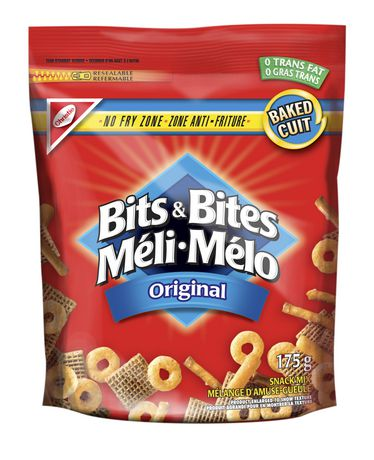
\includegraphics[height=3cm]{BitsandBites.jpg}};
\end{tikzpicture}
\end{frame}

\begin{frame}{Memory/Data Size}
\emph{Memory size} is a measure of memory storage capacity in bytes. It represents the \textit{maximum} capacity of data in the device.
\begin{example}
Given this flask, assume the red liquid is data and each mark represents 100 MB of data.  Select a true statement.
\begin{columns}[T] % align columns
\begin{column}{.0\textwidth}
\end{column}%
\begin{column}{.75\textwidth}
\begin{enumerate}[A)]
\item Memory size is 200 MB.
\item Flask can hold 0.5 GB of data.
\item Data size is about 200 KB.
\item Data size of 1000 KB would "overflow device".
\item All of the above statements are false.
\end{enumerate}
\end{column}%
\begin{column}{.24\textwidth}
\hspace*{-8mm}

\includegraphics[height=.3\textheight]{flask.png} 
\end{column}%
\end{columns}
\end{example}
\end{frame}

\begin{frame}<handout:0>
\begin{block}{Solution}
Given this flask, assume the red liquid is data and each mark represents 100 MB of data.  Select a true statement.
\begin{columns}[T] % align columns
\begin{column}{.0\textwidth}
\end{column}%
\begin{column}{.75\textwidth}
\begin{enumerate}[A)]
\item {
\color<beamer:1-|handout:0>{red}{Memory size is 200 MB.} \emph{$\sim$500MB}}
\item {\color<beamer:2-|handout:0>{ForestGreen}{Flask can hold 0.5 GB of data.}} 
\item {\color<beamer:3-|handout:0>{red}{Data size is about 200 KB.}} \only<beamer:3-|handout:0>\emph{$\sim$200 MB}
\item {\color<beamer:4-|handout:0>{red}{Data size of 1000 KB would "overflow device".}} 
\only<beamer:4-|handout:0>\emph{1000 KB = 1 MB < 500 MB}
\item {\color<beamer:5-|handout:0>{red}{All of the above statements are false.}}
\end{enumerate}
\end{column}%
\begin{column}{.24\textwidth}
\hspace*{-8mm}

\includegraphics[height=.3\textheight]{flask.png} 
\end{column}%
\end{columns}
\end{block}
\end{frame}





%https://learn.sparkfun.com/tutorials/analog-vs-digital/all
\begin{frame}{Analog vs. Digital: Thermometer example}
\begin{columns}[T] % align columns
\begin{column}{.1\textwidth}
\begin{center}
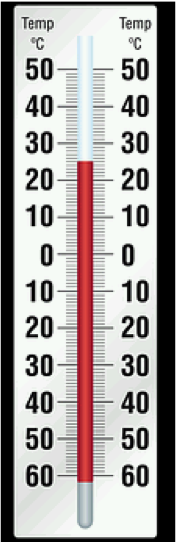
\includegraphics[height = 0.6\textheight]{thermo}
\end{center}
\end{column}%
\hfill%
\begin{column}{.8\textwidth}
\vspace{5mm}
A thermometer contains liquid which expands and contracts in response to temperature changes.\\[1em]\medskip
The liquid level is analog, and its expansion continuous over the temperature range.\\[1em]\medskip
This information can be represented using discrete units using digital
 thermometer, for example.
%By adding marks and units to the thermometer, we are digitizing the information.  
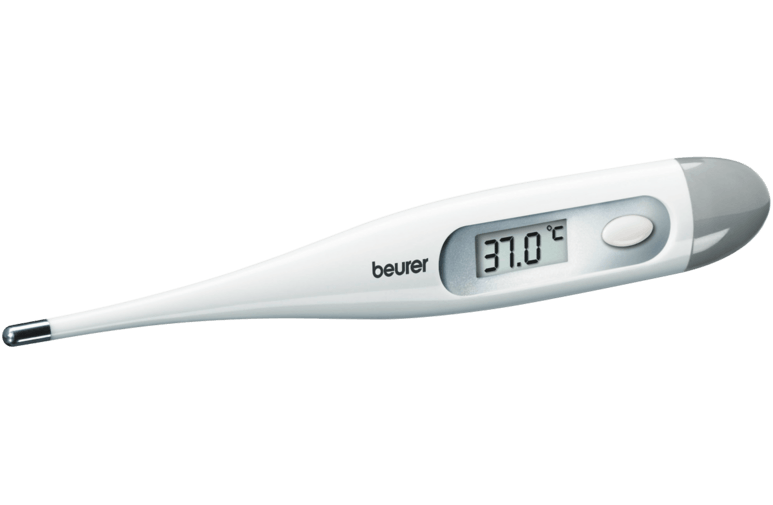
\includegraphics[width= 0.5\textheight]{img/dtheorm.png}
\end{column}%
\end{columns}
\end{frame}



\begin{frame}{Conversion of Analogue to Digital}
How would you digitize this analog data into 10 discrete points?
\begin{center}
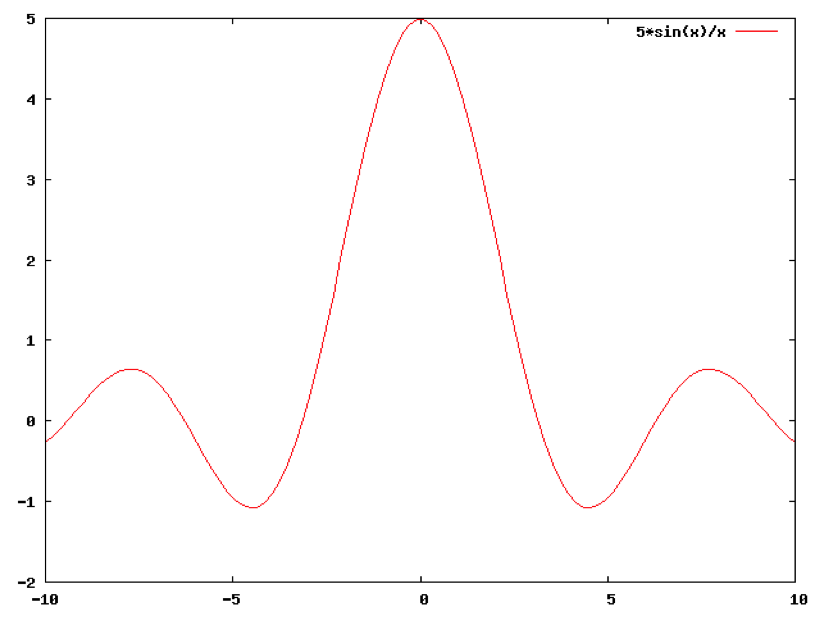
\includegraphics[height = 0.8\textheight]{Analog2Digital}
\end{center}
\end{frame}


\begin{frame}{Conversion of Analogue to Digital}
How would you digitize this analog data into 10 discrete points?
\begin{center}
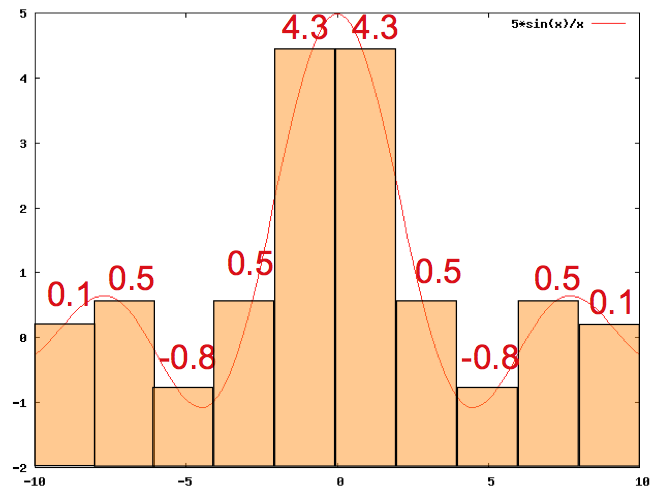
\includegraphics[height = 0.8\textheight]{Analog2DigitalB}
\end{center}
\end{frame}

\begin{frame}
{Why go digital over analogue?}
1) Computers are digital and many home electronics are
interfacing with computers.\eol
2) Analog signals are more susceptible to noise that degrades
the quality of the signal (sound, picture, etc.). The effect of
noise also makes it difficult to preserve the quality of analog
signals across long distances.\eol
3) Reading data stored in analog format is susceptible to data
loss and noise. Copying analog data leads to declining
quality
\end{frame}



\begin{frame}
%Fundamentally, computers use a numeral system that consist of only two possible values: 0 and 1.\eol
%A \emph{bit} is the smallest unit of storage and can either store a 0 or a 1\eol
%One \emph{byte}  represents a sequence of 8 bits.\\[1em] \medskip
%Computers convert these series of 0s and 1s into information.\medskip
A computer memory consists of billions of bits which allows for
an almost limitless number of possible states.\eol
 Bits are combined to allow more information to be
represented including characters and numbers
\begin{itemize}
\item eg. 0 = off, 1= on
\item {\tt 01100010} = ``b''\eol
\end{itemize}

To do this, it needs a set of rules on how to translate binary information into things like numbers, text, photos, video, etc.
\end{frame}

\begin{frame}{Bits and Bytes}
%Let's take a look at how a computer represents integers.\eol
Numbers are encoded in a computer using a fixed number of bits (usually 32 or 64).\medskip
\begin{center}
\begin{tabular}{|c|p{4.5cm}|c|}
\hline
 \bf \# &   & \bf \# of unique   \\
\bf  of bits & \bf Unique patterns & \bf  patterns  \\
\hline
{1} &{\tt 0, 1}  & $2^1 = 2$\\\hline
2 & {\tt 00, 01, 10, 11}& $2^2 = 4$\\\hline
\multirow{2}{*}{3} & {\tt 000, 001, 010, 100,}  & \multirow{2}{*}{$2^3 = 8$} \\
      &  {\tt 011, 101, 110,  111}&\\
     \hline
      \vdots & & \vdots \\     \hline
      32 & \dots & $2^{32} = 4,294,967,296$\\     \hline
       64 & \dots & $2^{64} > 18 $ quintillion\\
\hline
\end{tabular}
\medskip
\end{center}
The more bits you have, the more values you can represent.\eol
%A 32-bit register can store $2^{32}$ different values.

\end{frame}


\begin{frame}{Decimal System}
\begin{itemize}
\item Assuming we use a 32-bit register, we now need a way of mapping or converting these unique patterns of {\tt 0}s and {\tt 1}s to a specific meaning (in this case a number).
\medskip
\item A \emph{binary number} is a number expressed using only {\tt 0}s and {\tt 1}s (ie. in the base-2 numeral system or \emph{binary numeral system}).
\medskip
\item Before discussing the binary system, let's first discuss a  conversion system you should all be familiar with: the \emph{decimal system}
\end{itemize}

\end{frame}


\begin{frame}{Decimal System}
The decimal system uses digit placeholders, say \boxed{\phantom{9}}, that can take on values from the set  $\{0,1,2,3,4,5,6,7,8,9\}$\\ % numerical values between 0 and 9.\\
\medskip
The number of digits in the set is called the \emph{base}. So the base for this system is 10.\\
\medskip
Reading from right to left, the first placeholder represents ones, the second, 10s, the third hundreds, and so on \dots\\\medskip
We write eight million, two hundred ninety thousand, eight hundred forty one as:
\begin{center}
\boxed{{\uncover<1>{8}}}%
\boxed{{\uncover<1>{2}}}\boxed{{\uncover<1>{9}}}\boxed{{\uncover<1>{0}}}%
\boxed{{\uncover<1>{8}}}\boxed{{\uncover<1>{4}}}\boxed{{\uncover<1>{1}}}
\end{center}\medskip
%Each box above, can take on the values 0--9 (a choice of 10 digits) 
 $ = 8*10^6 + 2*10^5+ 9*10^4+ 0*10^3 + 8*10^2+ 4*10^1+ 1*10^0$
\end{frame}



\begin{frame}{Representing Data: Integers}
A \emph{binary system} works in the same way, only now, the placeholder must take a value from the set $\{0, 1\}$.\medskip

To put another way, instead of using base 10 wherein 
\begin{center}
ones=$10^0$, tens=$10^1$, hundreds=$10^2$, thousands=$10^3$, , etc.
\end{center}
we use base 2 where:
\begin{center}
 ones=$2^0$, `twos'=$2^1$, `fours'=$2^2$,  `eights'=$2^3$, etc. .
 \end{center}


For example, the integer 164 would be expressed as 
\begin{center}
\boxed{{\uncover<1->{\textcolor{ForestGreen}{1}}}}%
\boxed{{\uncover<2->{\textcolor{red}{0}}}}%
\boxed{{\uncover<1->{\textcolor{ForestGreen}{1}}}}%
\boxed{{\uncover<2->{\textcolor{red}{0}}}}%
\boxed{{\uncover<2->{\textcolor{red}{0}}}}%
\boxed{{\uncover<1->{\textcolor{ForestGreen}{1}}}}%
\boxed{{\uncover<2->{\textcolor{red}{0}}}}%
\boxed{{\uncover<2->{\textcolor{red}{0}}}}%
\end{center}

164 = 128 + 32 + 4\\
 \textcolor{ForestGreen}{$1\cdot2^7$} 
 + {\uncover<2->{\textcolor{red}{$0\cdot2^6$}}}   
 +  \textcolor{ForestGreen}{$1\cdot2^5$} 
+ {\uncover<2->{\textcolor{red}{$0\cdot2^4$}}}   
+z {\uncover<2->{\textcolor{red}{$0\cdot2^3$}}}   
+ \textcolor{ForestGreen}{$1\cdot2^2$}
+ {\uncover<2->{\textcolor{red}{$0\cdot2^0$}}}   
\end{frame}


\begin{frame}{Converting decimal to binary}
\label{dectobi}
There are a number of websites online (\href{https://www.rapidtables.com/convert/number/decimal-to-binary.html}{ex 1}, \href{https://binary-system.base-conversion.ro/convert-positive-unsigned-integers-from-decimal-system-to-unsigned-binary.php}{ex 2}) that can convert numbers from our decimal system (or simply decimal) to the binary system (or simply binary).
\medskip
However the steps to do it on paper are quite easy: 
% https://www.rapidtables.com/convert/number/decimal-to-binary.html
\begin{enumerate}
\item Divide the decimal number by 2.
\item Keep track of the integer quotient for the next iteration.
\item Keep track of the the remainder for the binary digit.
\item Repeat steps 1--3 until the quotient is equal to 0.
\item Construct the base 2 representation, by taking all the remainders starting from the bottom up.
\end{enumerate}
\medskip
Let's look at an example\dots
\end{frame}


\begin{frame}[t]\label{e37}
%% http://binary-system.base-conversion.ro/converted-positive-unsigned-integer-from-decimal-system-to-unsigned-binary.php?unsigned_integer_number_base_ten=37&unsigned_binary_base_2=100101
\begin{exampleblock}{Exercise}
Convert $37_{10}$ from base 10 (i.e decimal) to  binary base 2.
\end{exampleblock}
%{\color<beamer:1-|handout:0>{blue}{1. Divide the number repeatedly by 2.  Keep track of each remainder until we get a quotient that is equal to 0}}
\end{frame}


%\begin{frame}<handout:0>
%
%\end{frame}





\begin{frame}[t]\label{b132}
\begin{exampleblock}{Try it!}
Convert $132_{10}$ from base 10 (i.e decimal) to  binary base 2.
\end{exampleblock}
%See \href{http://binary-system.base-conversion.ro/convert-positive-unsigned-integers-from-decimal-system-to-unsigned-binary.php}{here} for solution
\end{frame}


\begin{frame}

\begin{block}{Question}
Does any see a problem with this system? \pause {\bf Hint:} this system is called \textit{unsigned binary}
\end{block}
\end{frame}

\begin{frame}{Representing Data: Integers}
Recall a 32-bit register can store $2^{32}$ different values.\medskip

The range of integer values it will represent depends on the \emph{encoding} type.\medskip
\begin{description}
\item[Unsigned Binary] Range is 0 through 4,294,967,295 =($2^{32}-1$)\medskip
\item[2's compliment] We use the first bit to store the sign (0=+, 1=-), so the range is -2,147,483,648 (-$2^{31}$) through 2,147,483,647 ($2^{31}$ - 1) .\medskip
%\item numbers are represented in \textit{two's complement notation}.  The "largest" bit pattern is -1.\medskip
% Midterm question: what is the range of integer values an 8bit (one-byte) binary number can hold? a number between 0 and 255
\end{description}
%\begin{exampleblock}
%{}Example: 123,456,789 as a binary 32-bit integer:
%\begin{center}
%\texttt{0}\texttt{0}\texttt{0}\texttt{0}\texttt{0}\texttt{1}\texttt{1}\texttt{1}
%\texttt{0}\texttt{1}\texttt{0}\texttt{1}\texttt{1}\texttt{0}\texttt{1}\texttt{1}
%\texttt{1}\texttt{1}\texttt{0}\texttt{0}\texttt{1}\texttt{1}\texttt{0}\texttt{1}
%\texttt{0}\texttt{0}\texttt{0}\texttt{1}\texttt{0}\texttt{1}\texttt{0}\texttt{1}
%\end{center}
%\end{exampleblock}
\end{frame}



\begin{frame}[fragile]{Representing Data: Real Numbers}
There are many standards for representing real numbers which include integers, rationals, fractions (eg -4,$\sqrt{2}$, 1/3) .  \\[1em]
The most common is \href{https://en.wikipedia.org/wiki/IEEE\_754}{IEEE 754} format which uses floating-point (FP) representation.\\[1em] %the most common
Similar to scientific notation, FP expresses real numbers using a base  and an exponent:  
\vspace{-5mm}
$$N = m * r^e$$ 
\vspace{-5mm}
 \begin{itemize} \setlength{\itemsep}{0pt}
 \vspace{-0.5cm}
\item $m$ = mantissa (the decimal component of a number)  % pronounced man-TEA-sa
\item  $e$ = exponent
\item  $r$ = radix \medskip% ramon uses r=2
%\item Note that converting from base 10 to base 2 is not always precise, since real numbers cannot be represented precisely in a fixed number of bits.
\end{itemize}
IEEE 754 adopts a binary FP where $r = 2$. \\ 
%(Sidenote: Scientific notation uses a decimal FP where $r=10$)  
\end{frame}
%






\begin{frame}{Representing Data: Doubles and Floats %\footnote{Photo sourced from: \cite{penjee}}
\href{https://blog.penjee.com/binary-numbers-floating-point-conversion/}{\tiny [Photo souce]}
}
Modern computers adopt \emph{IEEE 754}  for floating-point numbers % technical standard~
with two representation schemes: \medskip %32-bit single-precision and 64-bit double-precision.
\begin{description}
\item[{32 bit/{single-precision (or ``float')}}]1-bit sign; 8-bit exponent; 23-bit mantissa 
\hspace*{-15mm}
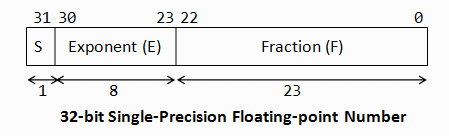
\includegraphics[width=0.8\textwidth]{DataRep_Float} \medskip
\item[{64 bit/{double-precision}}] 1-bit sign; 11-bit exp; 52-bit mantissa \medskip
\hspace*{-15mm}
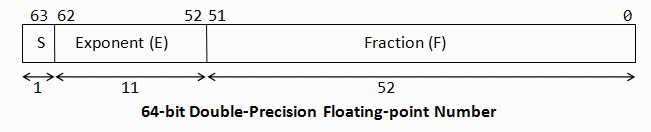
\includegraphics[width=0.8\textwidth]{DataRep_Double}
\end{description}

%A number with a decimal may be either stored as a \emph{double} (8 bytes) or \emph{float} (4 bytes).  Values are stored using a standard IEEE 754 format:
\end{frame}
%https://www.stat.berkeley.edu/~nolan/stat133/Spr04/chapters/representations.pdf


\begin{frame}
\begin{itemize}
\item As before, let's revisited a related concept (which we all would have learned about in high school)  to make this new concept easier to understand.
\medskip
\item Scientific notation operates in very much the same way as FP representation.
\medskip
\item Key features of normalized standard scientific notation:
\begin{itemize}
\item There is a single non-zero digit to the left of the decimal point
\item The power indicates how far we've moved the decimal point to the left (+ exponent) or right (- exponent)
\end{itemize}
\end{itemize}
\end{frame}





\begin{frame}{Representing Data: Normalized scientific notation}
\begin{exampleblock}
{Example: Normalized scientific notation:} The number 55,125.17 in normalized scientific notation is:
$${\color<1-|handout:1>{VioletRed}{5.512517}}\times {{\color<1-|handout:0>{brown}{10}}}^{{\color<1-|handout:1>{blue}{4}}}$$
\vspace{-0.5cm}
\end{exampleblock}
Key features of normalized standard scientific notation:
\begin{itemize}
\item 5.512517 is our {\color<1-|handout:1>{VioletRed}{mantissa}}
\item 4 is our {{\color<1-|handout:1>{blue}{exponent}}}
\item 10 is our {{\color<1-|handout:1>{brown}{radix}}}
\end{itemize}
\end{frame}


\begin{frame}{Representing Data: Normalized scientific notation}
\begin{exampleblock}
{Example: Normalized scientific notation:} The number 0.000 000 007 51 in normalized scientific notation is:
$${\color<1-|handout:1>{VioletRed}{7.51}}\times {{\color<1-|handout:0>{brown}{10}}}^{{\color<1-|handout:1>{blue}{-9}}}$$
\vspace{-0.5cm}
\end{exampleblock}
Key features of normalized standard scientific notation:
\begin{itemize}
\item 7.51 is our {\color<1-|handout:1>{VioletRed}{mantissa}}
\item -9 is our {{\color<1-|handout:1>{blue}{exponent}}}
\item 10 is our {{\color<1-|handout:1>{brown}{radix}}}
\end{itemize}
\end{frame}

\begin{frame}{Converting decimal fraction to binary - Phase 1}
\begin{enumerate}
\item Convert the integer part of decimal to binary (as on \hyperlink{dectobi}{this} slide)\label{step1}
\item Convert the fractional part of decimal to binary equivalent\label{step2}
\vspace{-1em}
\begin{enumerate}[i)]
\item \textit{Multiply} the fractional part by 2.
\item Keep track of the integer part for the binary digit
\item Keep track of the fractional part for the next iteration
\item Repeat steps 1--3 until the fractional part is equal to 0 or we have enough digits to fill the mantissa
\item Construct the base 2 representation, by taking all the \textit{integer} parts \textit{starting from the top}
\end{enumerate}
\item Write the result from step \ref{step1} to the left of the decimal and the result from step \ref{step2} to the right of the decimal. \label{step3}
\end{enumerate}
\end{frame}

\begin{frame}{Converting decimal fraction to binary - Phase 2}
\begin{enumerate}
\setcounter{enumi}{3}
\item Normalize the result from step \ref{step3} by shifting the decimal (either left or right) so that only one non zero digit remains to the left of the decimal. The number of places we shift will determine our exponent\label{step5}
\item Adjust the exponent by adding  $2^{(8-1)} - 1$ to the exponent \label{step6}
\item Convert the result in step \ref{step6} to to binary (as on \hyperlink{dectobi}{this} slide)\label{step7}
\item Construct the binary number: \label{finalstep}
\begin{enumerate}[i)]
\item Fill in the sign bit (0 = positive, 1 = negative)
\item Fill in the exponent bits with the result from step \ref{step7}
\item Fill in the mantissa with the first 23 digits to the right of the decimal from step \ref{step5}
\end{enumerate}

\end{enumerate}
\end{frame}



\begin{frame}{Representing Data: Doubles and Floats}
\begin{exampleblock} 
{Example: 32-bit single precision} The number -37.17 stored as 4 consecutive bytes is: 
\vspace{-2mm}
\begin{center}
\hspace{-20mm}\green{sign} \quad   \blue{exponent} \quad\quad \quad\qquad \yellow{mantissa}\\
\texttt{\green{1} \blue{1000 0100} \yellow{001 0100 1010 1110 0001 0100}}
\end{center} 
\end{exampleblock}
{\bf Step \ref{step1})} Convert the number to binary scientific notation%/Fractional Binary
\begin{itemize}
\item Integer part (37) in binary \textcolor{orange}{\tt 100101} % {\small (typical to exclude leading 0s)}
(as shown in the \hyperlink{e37}{previous exercise})
%\item The fractional part (0.17) in binary is
%\newline {\tt 0.0010 1011 1000 0101 0001 1110 10}
\end{itemize}
%$$37.17_{10} =  {\tt 10 0101.0010 1011 1000 0101 0001 1110 10}_2$$
\end{frame}

\frame[t]{
%http://binary-system.base-conversion.ro/real-number-converted-from-decimal-system-to-32bit-single-precision-IEEE754-binary-floating-point.php?decimal_number_base_ten=0.17&sign=0&exponent=01111100&mantissa=01011100001010001111010
%\begin{exampleblock}{Exercise}
%Convert 0.17 to binary.
%\end{exampleblock}
{\bf Step \ref{step2})  \footnotesize{Convert the fractional part of decimal to binary equivalent}}

\begin{columns}
\begin{column}{0.5\textwidth}
\vspace{-5mm}
   \small
\begin{table}[htdp]
\begin{center}
\begin{tabular}{rl}
1) 0.17 * 2  = \textcolor{MediumSlateBlue}0 + 0.34 \\
2) 0.34 * 2 = \textcolor{MediumSlateBlue}0 + 0.68\\
3) 0.68 * 2 = \textcolor{MediumSlateBlue}1 + 0.36\\
4) 0.36 * 2 = \textcolor{MediumSlateBlue}0 + 0.72\\
5) 0.72 * 2 = \textcolor{MediumSlateBlue}1 + 0.44\\
6) 0.44 * 2 = \textcolor{MediumSlateBlue}0 + 0.88\\
7) 0.88 * 2 = \textcolor{MediumSlateBlue}1 + 0.76\\
8) 0.76 * 2 = \textcolor{MediumSlateBlue}1 + 0.52\\
9) 0.52 * 2 = \textcolor{MediumSlateBlue}1 + 0.04\\
10) 0.04 * 2 = \textcolor{MediumSlateBlue}0 + 0.08\\
11) 0.08 * 2 = \textcolor{MediumSlateBlue}0 + 0.16\\
12) 0.16 * 2 = \textcolor{MediumSlateBlue}0 + 0.32\\
\dots continuted
\end{tabular}
\end{center}\
\end{table}%
\end{column}
\begin{column}{0.5\textwidth}  %%<--- here
\vspace{-10mm}
\small
\begin{table}[htdp]
\begin{center}
\begin{tabular}{rl}
\dots\\
13) 0.32 * 2 = \textcolor{MediumSlateBlue} 0 + 0.64\\
14) 0.64 * 2 = \textcolor{MediumSlateBlue}1 + 0.28\\
15) 0.28 * 2 = \textcolor{MediumSlateBlue}0 + 0.56\\
16) 0.56 * 2 = \textcolor{MediumSlateBlue}1 + 0.12\\
17) 0.12 * 2 = \textcolor{MediumSlateBlue}0 + 0.24\\
18) 0.24 * 2 = \textcolor{MediumSlateBlue}0 + 0.48\\
19) 0.48 * 2 = \textcolor{MediumSlateBlue}0 + 0.96\\
20) 0.96 * 2 = \textcolor{MediumSlateBlue}1 + 0.92\\
21) 0.92 * 2 = \textcolor{MediumSlateBlue}1 + 0.84\\
22) 0.84 * 2 = \textcolor{MediumSlateBlue}1 + 0.68\\
23) 0.68 * 2 = \textcolor{MediumSlateBlue}1 + 0.36\\
24) 0.36 * 2 = \textcolor{MediumSlateBlue}0 + 0.72\\
\dots continued
\end{tabular}
\end{center}
\end{table}%
\end{column}
\end{columns}
\vspace{-5mm}
We didn't (and won't) get a fractional part equal to zero but since we have enough iterations to fill the mantissa %and at least one integer that was different from zero => FULL STOP (losing precision...)
we can stop. $0.17_{10} =
{\tt 0.\textcolor{MediumSlateBlue}{0010 1011 1000 0101 0001 1110}\dots}_2$

}


%\begin{frame}<handout:0>
%
%\end{frame}


\begin{frame}{}{}

{\bf Step \ref{step3}:}
Write the \textcolor{orange}{result from step \ref{step1}} to the left of the decimal and the \textcolor{MediumSlateBlue}{result from step \ref{step2}} to the right of the decimal. 
$$
{\tt \textcolor{orange}{37}.\textcolor{MediumSlateBlue}{17}_{10}} =  {\tt \textcolor{orange}{10 0101}.\textcolor{MediumSlateBlue}{0010 1011 1000 0101 0001 1110 10}}_2
$$
{\bf Step \ref{step5}:} Normalize the result from step \ref{step3} by shifting the decimal (either left or right) so that only one non zero digit remains to the left of the decimal (form {\tt 1.xxxxxx}).  
\begin{align*}
 & =  {\tt 1\red{0 0101}.0010 1011 1000 0101 0001 1110 10}_2\\
&= {\tt 1.{0 01010010 1011 1000 0101 00} 01 1110 10}_2 \times 2^{\red{5}}
\end{align*}

Since decimal moved 5 spaces to the left, the exponent becomes (positive) 5.

\end{frame}

\begin{frame}{}{}
{\bf Step \ref{step6}} Adjust the exponent by adding  $2^{(8-1)} - 1$ to the exponent 
$$
{\tt 5} \text{ becomes } 5 + 2^{(8-1)} - 1 = 132
$$
{\bf Step \ref{step7}} Convert the result in step \ref{step6} to to unsigned binary (done on \hyperlink{b132}{this} slide)
$${\tt 132}_{10} = {\tt 1000\ 0100}_{2}$$
\end{frame}


\begin{frame}{Why the exponent adjustment?}
\begin{center}
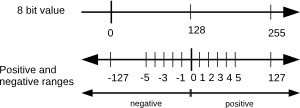
\includegraphics[width=0.5\textwidth]{img/binary-floating-point-8-bit-range.png}
\href{https://blog.penjee.com/binary-numbers-floating-point-conversion/}{\tiny [Photo souce]}
\end{center}
The 8-bits set aside for the exponent can represent $2^8=256$ different values (0-- 255 using unsigned binary) 
\medskip

However, had the decimal moved to the \textit{right}, the exponent would have been a negative number.
\medskip

To accommodate negative integers in unsigned binary system we simply allow he lower half of the range (0--127) to be used for negative exponents and the upper other half (128--255) will be used for positive exponents. 
\end{frame}

\begin{frame}{Why the exponent adjustment?}
\begin{center}
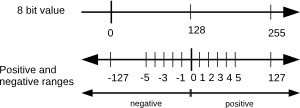
\includegraphics[width=0.5\textwidth]{img/binary-floating-point-8-bit-range.png}
\href{https://blog.penjee.com/binary-numbers-floating-point-conversion/}{\tiny [Photo souce]}
\end{center}
\begin{itemize}
\item Our unadjusted positive exponent (eg 5) is now adjusted to $5+(2^{8 -1} - 1) = 5 + 127 =132_{10} =  {\tt 1000\ 0100}_{2}$.
\item To provide another examples:
\vspace{-1.2em}
\begin{center}
\begin{tabular}{rrl}
-8 is represented as  &-8 + 127 = 119$_{10}$& = {\tt 01110111}$_2$\\
 0 is represented as & 0 + 127 = 127$_{10}$ &= {\tt 01111111}$_2$\\
 +1 is represented as& +1 + 127 = 128$_{10}$ &= {\tt 10000000}$_2$
\end{tabular}
\end{center}
%\begin{itemize}
% \item -8 is represented as -1 + 127 = 119 = {\tt 01110111}$_2$
%%\item -1 is represented as -1 + 127 = 126 = {\tt 01111110}_2
%\item 0 is represented as  0 + 127 = 127 = {\tt 01111111}$_2$
%\item +1 is represented as +1 + 127 = 128 = {\tt 10000000}$_2$
%\end{itemize}
% if our exponent happened to be  -8, we would calculate our 8-bit exponent using:  $-8+(2^{8 -1} - 1)= -8+ 127=119_{10} = {\tt 0111\ 0111}_2$
%\item Now we convert $132_{10}$ to the 8-bit value of ${\tt \blue{1000 0100}}_2$.
\item This scheme (called \href{https://en.wikipedia.org/wiki/Offset_binary\#Excess-127}{Excess-127}) supports unadjusted exponents of -127 to 128
\end{itemize}
%N.B. An unadjusted  negative exponent (eg. -8) would have an 8-bit value of $-8+127=119_{10} = {\tt 1110111}_2$
\end{frame}

\begin{frame}{}{}
\begin{exampleblock} 
{Example: 32-bit single precision} The number -37.17 stored as 4 consecutive bytes is: 
\vspace{-2mm}
\begin{center}
\hspace{-20mm}\green{sign} \quad   \blue{exponent} \quad\quad \quad\qquad \yellow{mantissa}\\
\texttt{\green{\boxed{1}} \blue{ \boxed{\phantom{1000 0100}}} \yellow{\boxed{\phantom{001 0100 1010 1110 0001 0100}}}}
\end{center} 
\end{exampleblock}
{\bf Step  \ref{finalstep}} Construct the binary number:
\begin{enumerate}[i)]
\item Fill in the sign bit (0 = positive, 1 = negative)
\begin{itemize}
\item since -37.17 is a negative number the first bit = 1.
\end{itemize}
%\item Fill in the exponent bits with the result from step \ref{step7}
%\item Fill in the mantissa with the first 23 digits to the right of the decimal from step \ref{step5}
\end{enumerate}
\end{frame}


\begin{frame}{}{}
\begin{exampleblock} 
{Example: 32-bit single precision} The number -37.17 stored as 4 consecutive bytes is: 
\vspace{-2mm}
\begin{center}
\hspace{-20mm}\green{sign} \quad   \blue{exponent} \quad\quad \quad\qquad \yellow{mantissa}\\
\texttt{\green{\boxed{1}} \blue{ \boxed{{\tt 1000\ 0100}}} \yellow{\boxed{\phantom{001 0100 1010 1110 0001 0100}}}}
\end{center} 
\end{exampleblock}
{\bf Step  \ref{finalstep}} Construct the binary number:
\begin{enumerate}[ii)]
%\item Fill in the sign bit (0 = positive, 1 = negative)
%\begin{itemize}
%\item since -37.17 is a negative number the first bit = 1.
%\end{itemize}
\item Fill in the exponent bits with the result from step \ref{step7}
\begin{itemize}
\item Recall our unadjusted positive exponent (eg 5) was adjusted to $5+(2^{8 -1} - 1) = 5 + 127 =132_{10} =  {\tt 1000\ 0100}_{2}$.
\end{itemize}
%\item Fill in the mantissa with the first 23 digits to the right of the decimal from step \ref{step5}
\end{enumerate}
\end{frame}


\begin{frame}{}{}
\begin{exampleblock} 
{Example: 32-bit single precision} The number -37.17 stored as 4 consecutive bytes is: 
\vspace{-2mm}
\begin{center}
\hspace{-20mm}\green{sign} \quad   \blue{exponent} \quad\quad \quad\qquad \yellow{mantissa}\\
\texttt{\green{\boxed{1}} \blue{ \boxed{{\tt 1000\ 0100}}} \yellow{\boxed{{\tt 001\ 0100\ 1010\ 1110\ 0001\ 0100}}}}
\end{center} 
\end{exampleblock}
{\bf Step  \ref{finalstep}} Construct the binary number:
\begin{enumerate}[iii)]
%\item Fill in the sign bit (0 = positive, 1 = negative)
%\begin{itemize}
%\item since -37.17 is a negative number the first bit = 1.
%\end{itemize}
%\item Fill in the exponent bits with the result from step \ref{step7}
%\begin{itemize}
%\item Recall our unadjusted positive exponent (eg 5) was adjusted to $5+(2^{8 -1} - 1) = 5 + 127 =132_{10} =  {\tt 1000\ 0100}_{2}$.
%\end{itemize}
\item Fill in the mantissa with the first 23 digits to the right of the decimal from step \ref{step5}
\newline \yellow{\sout{\tt 1.}{\tt
%10101110 10101010 0101011 \sout{1000 0101 0001 1110}}}
00101001010111000010100\sout{01111010}}}
\end{enumerate}
%\vfill
%See an \href{http://binary-system.base-conversion.ro/convert-real-numbers-from-decimal-system-to-32bit-single-precision-IEEE754-binary-floating-point.php}{online converter for -37.17}
\end{frame}

% -3.71699981689453125E1
% 1 1000 0100 001 0100 1010 1110 0001 0100

\begin{frame}{Precision}
Take note of the fact that we deleted some information in order to get the number -37.17 to fit into the 32-bit single representation. 
\medskip

As a result,  the storage of this number is -37.1699981689453125.
  \begin{alertblock}{Lack of precision}
Rounding errors will occur since some real numbers will 
%not have exact representation (Can only exactly represent numbers of the form x/2k)
%since real numbers cannot be represented precisely in a fixed number of bits.
%%cannot be represented precisely in a fixed number of bits.
%Other rational numbers
 have repeating bit representations.  This lack of precision may be important in scientific applications!
%Note that converting from base 10 to base 2 is not always precise, 
%Can only exactly represent numbers of the form x/2k
  \end{alertblock}

\end{frame}


\begin{frame}{Precision}
Rational numbers of the form $x/2^k$, where $x$ and $k$ are integers, can have exact fractional binary representation\\[1em]\medskip

For example:
\begin{itemize}
\item  $0.015625 = 1/2^6$, $-1.5 = -3/2$, $96 = 3/2^{-5}$ will have exact representation.\medskip
\item   $0.1, 123.4, 0.025$ will not have exact representation.
\end{itemize}

\end{frame}

\begin{frame}[t]
\begin{block}{Try It! You can check your answer \href{http://binary-system.base-conversion.ro/convert-real-numbers-from-decimal-system-to-32bit-single-precision-IEEE754-binary-floating-point.php}{here}.}
Convert 0.015625 to 32 bit single precision.
\end{block}
{\bf Step \ref{step1}}  Convert the integer part of decimal to binary 
\vfill
{\bf Step \ref{step2}} Convert the fractional part of the decimal to binary 

\vfill
\vfill

\end{frame}

\begin{frame}[t]{}{}
{\bf Step \ref{step3}}  Write the result from step \ref{step1} to the left of the decimal and the result from step \ref{step2} to the right of the decimal.\newline
{\bf Step \ref{step5}}  Normalize the result from step \ref{step3}\
\vfill
\end{frame}


\begin{frame}[t]{}{}
{\bf Step \ref{step6}}  Adjust the exponent by adding  $2^{(8-1)} - 1$ to the exponent 
{\bf Step \ref{step7}}  Convert the result in step \ref{step6} to to binary 
\end{frame}

\begin{frame}[t]{}{}
{\bf Step \ref{finalstep}}  Construct the binary number: 
\begin{enumerate}[i)]
\item Fill in the sign bit (0 = positive, 1 = negative)
\item Fill in the exponent bits with the result from step \ref{step7}
\item Fill in the mantissa with the first 23 digits to the right of the decimal from step \ref{step5}
\end{enumerate}

\end{frame}


\begin{frame}{Comment}
\begin{itemize}
\item While 64-bit can accommodate a wider range of number as shown in the table below, in most scenarios, you will be fine using 32-bit.
%\item The range and accuracy are both much better than with a float and the extra memory used for double is not noticeable unless you are building a very large data structure.
\begin{table}[htdp]
\caption{Source: \href{https://chortle.ccsu.edu/java5/Notes/chap11/ch11_2.html}{here}}
\begin{center}
\begin{tabular}{|c|c|c|}
\hline
Type	& Size	& Range\\
\hline
float & 	32 bits	& -3.4E+38 to +3.4E+38\\
double&	64 bits	& -1.7E+308 to +1.7E+308\\
\hline\end{tabular}
\end{center}
\label{default}
\end{table}%
\end{itemize}
\end{frame}

\begin{frame}{Hexadecimal}
We saw how binary and decimal systems consist of two and ten digits respectively.\eol
For that reason, binary is also known as \emph{base 2} and decimal as \emph{base 10}.\eol
\alert{Hexadecimal} is another such system that contains sixteen digits and is therefore known as \emph{base 16}.\eol
Like decimal, hexadecimal uses the same 10 digits ({\tt 0---9})\eol
In addition, it uses: {\tt A,B,C,D,E}, and \tt F.
\end{frame}

% Sources of info:
%http://computingvoyage.com/328/an-introduction-to-bits-bytes-and-hexadecimal/



\begin{frame}
\vspace{-1em}
\begin{center}
\small
\texttt{
\begin{tabular}{|c|c|l|}
\hline
Hexadecimal & Decimal & Binary\\
Base 16	& Base 10	 & Base 2\\\hline
0&	0&	0\\
1&	1&	1\\
2&	2&	10\\
3&	3&	11\\
4&	4&	100\\
5&	5&	101\\
6&	6&	110\\
7&	7&	111\\
8&	8&	1000\\
9&	9&	1001\\
A&	10&	1010\\
B&	11	&1011\\
C&	12&	1100\\
D&	13&	1101\\
E&	14&	1110\\
F&	15&	1111\\\hline
\end{tabular}}
\end{center}
\end{frame}

\begin{frame}
Notice, it takes 4 binary digits (a nibble) to represent a single hexadecimal digits. \eol
Consequently, hexadecimal provides a compact short hand for binary.\eol
Another benefit for using hexadecimal is that it is easier (for a human) to read. \eol
The most common place to see this hexadecimal notation is when describing colours, eg.
\begin{center}
Roses are \red{\tt \#FF0000} (in decimal (255, 0, 0))\\
Violets are \blue{\tt \#0000FF} (in decimal (0, 0, 255))
\end{center}
%N.B. Because each of the three colors can have values from 0 to 255 (256 possible values), there are:
%256 * 256 * 256 
% 	= 16,777,216 possible color combinations

\end{frame}

%\begin{frame}[t]
%%https://www.permadi.com/tutorial/numDecToHex/
%% http://decimal-to-binary.com/decimal-to-binary-converter-online.html?id=818
%\begin{example}
%Convert 2000 from decimal to hexadecimal 
%\end{example}
%\end{frame}
%
%\begin{frame}[t]
%\begin{example}
%Convert D301 hexadecimal to binary
%\end{example}
%\end{frame}
%
%\begin{frame}[t]
%\begin{example}
%Convert this binary sequence to hexadecimal:\\
%{\tt 0000 0101 1000 0001 1111 1110}
%\end{example}
%\end{frame}


\begin{frame}{Representing Data: Characters}
A character is mapped to a sequence of bits using a \textit{lookup or translation table}.  \\[1em]\medskip

A common encoding is \emph{ASCII} (American Standard Code for Information Interchange), which uses 8 bits to represent characters.\\[1em] \medskip
\begin{center}
 \begin{tabular}{|c|c|}
 \hline
{\bf bits}	& {\bf character}\\
 \hline
{\tt 01000001}	&A\\
{\tt 01000010}	&B\\
{\tt 01000011}	&C\\
{\tt 01000100}	&D\\
{\tt 01000101}	&E\\
{\tt 01000110}	&F\\
\dots & \dots
    \end{tabular}
\end{center}
%ASCII originally used 7 bits to represent each character, allowing for 128 unique characters
\end{frame}




\begin{frame}{Representing Data: Characters}
\begin{columns}[T] % align columns
\begin{column}{.2\textwidth}
\vspace{0.4\textheight}
\begin{flushright}
First 4 bits
\end{flushright}
\end{column}%
\hfill%
\begin{column}{.8\textwidth}
\vspace{-1em}
\qquad \qquad\qquad \quad Next 4 bits\\[1em]
 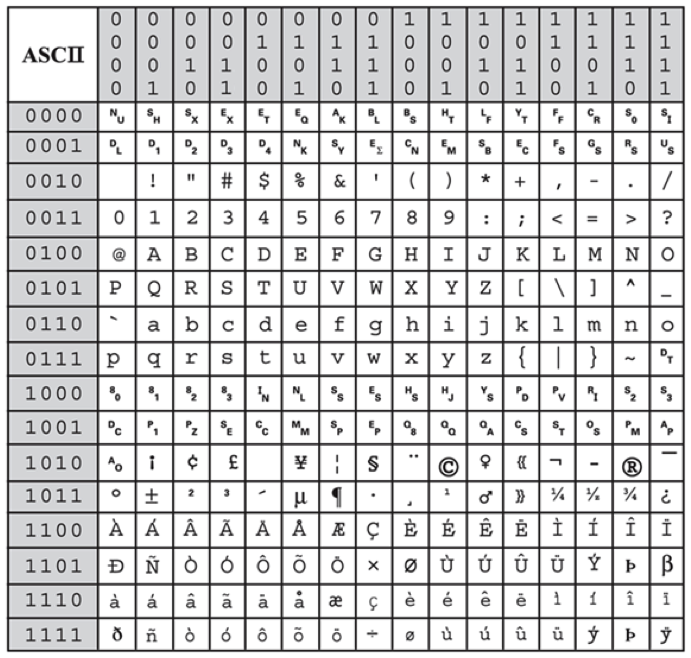
\includegraphics[height=0.73\textheight]{ASCIITable}
\end{column}%
\end{columns}
\medskip
\begin{exampleblock}{}
Exercise: Try writing your name in ASCII!
\end{exampleblock}
\end{frame}
%For the more advanced students, notes:
%Note how the last 4 digits of ASCII encoding of numbers is equivalent to their decimal representation.  eg. 4 = 0011 0100
%Note how upper and lower case letters only differ in first 4 bits.  Lower 4 bits are identical.  A = 0100 0001  and a = 0110 0001
%The dash is at 45 or 00101101.  That is what you get when you type minus or dash on keyboard.  Not sure how to get dash at 1010 1100.


\begin{frame}{Representing Data: Characters}
\begin{example}
 What ASCII character is 0100 0101?
\begin{enumerate}[A)]
 \item T
\item !
 \item @
\item E
 \end{enumerate}
\end{example}
\end{frame}
% Answer D) E.

\begin{frame}<handout:0>{Representing Data: Characters}
\begin{block}
{Answer:}
 What ASCII character is 0100 0101?
\begin{enumerate}[A)]
 \item A
\item !
 \item @
\item \yellow{\it E}
 \end{enumerate}
\end{block}
\end{frame}


\begin{frame}{ASCII Encoding}
\begin{example}
What is ``Test'' encoded in ASCII?
\begin{enumerate}[A)]
 \item {\tt 01110100 01100101 01110011 01110100}
\item {\tt 01010100 01100101 01110011 01110100}
 \item {\tt 01000101 01010110 00110111 01000111}
\item {\tt 01010100 01000101 01010011 01010100}
 \end{enumerate}
\end{example}
\end{frame}



\begin{frame}<handout:0>{ASCII Encoding}
\begin{block}
{Answer:}
What is ``Test'' encoded in ASCII?
\begin{enumerate}[A)]
 \item {\tt 01110100 01100101 01110011 01110100}
\item \yellow{\it 01010100 01100101 01110011 01110100}
 \item {\tt 01000101 01010110 00110111 01000111}
\item {\tt 01010100 01000101 01010011 01010100}
 \end{enumerate}
\end{block}
\end{frame}




\begin{frame}
\begin{itemize}
\item While these conversions are useful to see,  these conversions need not be done `by hand'.
\medskip
\item If there was a time when we need to see these conversions, there are countless sites available online for doing so, eg. \href{http://www.binaryhexconverter.com/ascii-text-to-binary-converter}{ASCII to Binary}
\medskip
\end{itemize}
\begin{block}{Limitations with ASCII?}
Does anyone see a problem with using ASCII as a character encoding?
\end{block}\pause
Although ASCII is suitable for English text, many world languages, including Chinese, require a larger number of symbols to represent their basic alphabet.

\end{frame}

%
%\begin{frame}<handout:0>{ASCII Encoding}
%\begin{block}
%{Answer:}
%What is ``Test'' encoded in ASCII?
%\begin{enumerate}[A)]
% \item {\tt 01110100 01100101 01110011 01110100}
%\item \yellow{\tt 01010100 01100101 01110011 01110100}
% \item {\tt 01000101 01010110 00110111 01000111}
%\item {\tt 01010100 01000101 01010011 01010100}
% \end{enumerate}
%\end{block}
%\only<1>{Quick link:  \url{http://www.binaryhexconverter.com/ascii-text-to-binary-converter}}
%\end{frame}

\begin{frame}{Representing Text Beyond ASCII - Unicode}
% http://www.differencebetween.net/technology/software-technology/difference-between-unicode-and-ascii/
The \emph{Unicode} standard uses patterns of 16-bits (2 bytes) to represent the major symbols used in all languages.\medskip
\begin{itemize}
\item First 256 characters exactly the same as ASCII.
\item Maximum number of symbols: 65,536.
\end{itemize}
\vfill
Unicode can be implemented by different character encodings (eg.  UTF-8, UTF-16, UTF-32) with new versions released on a regular basis.
\vfill
UTF-8, the dominant encoding on the World Wide Web (used in over 92\% of websites). 
\vfill
 As of May 2019 the most recent version, Unicode 12.1, contains  137,994 characters covering 150 modern and historic scripts, as well as multiple symbol sets and emojis. 
\includegraphics[width=1em]{img/yay}.
\vfill
\end{frame}


%\begin{frame}{Aside: Character Fonts}
%When a character is displayed on a screen, a particular font is used.\\[1em]\medskip
%
%The font is how to present the data (the character).\\[1em]\medskip
%
%Note that the font itself is data where each character has a mapping to a sequence of bytes representing pixels (image) on how to draw the character.
%\end{frame}

% https://en.wikipedia.org/wiki/String_(computer_science)#Byte-_and_bit-terminated
\begin{frame}{Representing Data: Strings}
% http://cglab.ca/~morin/teaching/5408/notes/strings.pdf
A string is a sequence of characters  allocated in consecutive
memory bytes.  \\[1em]\medskip
A string has a terminator to know when it ends:\\[1em]\medskip
\begin{itemize}
\item
\begin{description}
\item[Null-terminated string] last byte value is `$\backslash$0' to indicate end of string.\medskip
\end{description}
\item
\begin{description}
\item[length-prefixed] length of string in bytes is specified (usually in the first few bytes before string starts).
\end{description}
\end{itemize}
\end{frame}



\setbeamersize{description width=0.5cm}
\begin{frame}{Representing Data: Dates and Times}
A \emph{date} value can be represented in multiple ways:\medskip
\begin{description}
\item[Integer representation] number of days past since a given date \medskip
\begin{itemize}
\item Example: Julian Date (astronomy) -- number of days since noon, January 1, 4713 BC. \href{https://en.wikipedia.org/wiki/Julian\_day\#History}{Why this date?}\medskip
% why julian? http://curious.astro.cornell.edu/about-us/125-observational-astronomy/timekeeping/calendars/763-how-was-the-starting-point-for-the-julian-date-system-chosen-advanced
% where 3 cycles converge, plus no use for negative years
\end{itemize}
\item[String representation] represent a date's components (year, month, day) as individual characters of a string\medskip
\begin{itemize}
\item Example: YYYYMMDD or YYYYDDD
\end{itemize}
\end{description}
%Please do not reinvent Y2K by using YYMMDD!!
\end{frame}

\begin{frame}{Representing Data: Dates and Times}
A \emph{time} value can also be represented in similar ways:\medskip
\begin{description}
\item [Integer representation] number of sec since a given time\medskip
\begin{itemize}
\item  Example: Number of seconds since Thursday, January 1, 1970 (UNIX) %\only<beamer:2-|handout:0>{(Year 2038 problem)}\medskip\medskip
\end{itemize}
\item [String representation] hours, minutes, seconds, fractions\medskip
\begin{itemize}
\item Example: HHMMSSFF\
\end{itemize}
\end{description}
\medskip
Read \href{https://en.wikipedia.org/wiki/Year_2038_problem}{here} about the year 2038 problem (analogy to the Y2K problem).
\end{frame}
%The year 2038 problem (also known as Unix Millennium Bug, Y2K38 or Y2.038K by analogy to the Y2K problem) 
%may cause some computer software to fail before or in the year 2038. The problem affects all software and systems that both store system time as a signed 32-bit integer, and interpret this number as the number of seconds since 00:00:00 UTC on Thursday, 1 January 1970.[1] The furthest time that can be represented this way is 03:14:07 UTC on Tuesday, 19 January 2038.[2] Times beyond this moment will "wrap around" and be stored internally as a negative number, which these systems will interpret as a date in 1901 rather than 2038. This will likely cause problems for users of these systems due to erroneous calculations
%
%Julian Date: number of days since noon, January 1, 4713 BC
%
%Question: Why since January 1, 1970? Cannot find a good answer except that was just what was chosen.
%

\begin{frame}{Encoding other data}
We have seen how we can encode characters, numbers, and strings using only sequences of bits (and translation tables).\\[1em]\medskip

The documents, music, and videos that we commonly use are much more complex.  However, the principle is exactly the same.  We use sequences of bits and \emph{interpret} them based on the \emph{context} to represent information.\\[1em]\medskip

As we learn more about representing information, always remember that everything is stored as bits, it is by interpreting the context that we have information.
\end{frame}


\begin{frame}{Metadata}
\emph{Metadata} is data that describes other data.\\[1em]\medskip
Examples of metadata include: \medskip
\begin{itemize}
\item names of files\medskip
\item column names in a spreadsheet\medskip
\item table and column names and types in a database\\[1em]\medskip
\end{itemize}
Metadata helps you understand how to interpret and manipulate the data.
\end{frame}

\begin{frame}{Files}
A \emph{file} is a sequence of bytes on a storage device.\medskip
\begin{itemize}
\item A file has a name.\medskip
\item A computer reads the file from a storage device into memory to use it.\\[1em]\medskip
\end{itemize}

The operating system manages how to store and retrieve the file bytes from the device. \\[1em]\medskip

The program using the file must know how to interpret those bytes based on its information (e.g. metadata) on what is stored in the file.
\end{frame}

\begin{frame}{File Encoding}
A file \emph{encoding} is how the bytes represent data in a file.\\[1em]\medskip
%  is how data is convert into a coded form, while
% a character encoding describes how bits are translated into characters %https://www.youtube.com/watch?v=HGitnaoVQ-A

A file encoding is determined from the file extension (e.g. .txt or .xlsx) which allows the operating system (OS)  to know how to process the file.\\[1em]\medskip
The extension allows the OS to select the program to use.  The program understands how to process the file in its format.
\end{frame}


% https://dev.to/sharkdp/what-is-a-binary-file-2cf5
% At a generic level of description, there are two kinds of computer files: text files and binary files.[1]
% https://perlmaven.com/what-is-a-text-file   In general every file is a binary file, but if the data in it contains only text (letter, numbers and other symbols one would use in writing, and if it consists of lines, then we consider it a text file.

\begin{frame}{\href{https://www.nayuki.io/page/what-are-binary-and-text-files}{Binary vs Text files}}
\begin{itemize}
\item At a generic level of description, there are two kinds of computer files: text files and binary files.\medskip
\item The difference between binary and text files is in how these bytes are interpreted. \medskip
\item A text file is a file encoded in a character format such as ASCII or Unicode.  These files are readable by humans.\medskip
\item Data analytics will often involve processing text files.\medskip
\item We can usually tell if a file is binary or text based on its file extension.

\end{itemize}

\end{frame}



\begin{frame}{File Encodings: Text Files}

There are many different text file encodings:\medskip
\begin{itemize}
\item \emph{Web standards}: html, xml, css, svg, json, ...
\begin{itemize}
\item \emph{JSON file} data encoded in JSON (\emph Java\emph{S}cript \emph Object \emph Notation) format \medskip
% JSON formal is a syntax for storing and exchanging data \medskip
\item \emph{XML file} data encoded in XML (Extensible Markup Language) format\medskip
\end{itemize}
\item \emph{Tabular data}: csv, tsv, \dots 
\begin{itemize}
\item \emph{CSV comma-separate file} each line is a record, fields separated by commas\medskip
\item \emph{tab-separated file}  each line is a record, fields separated by tabs\medskip
\end{itemize}
% They are two formats of representation of information. While JSON was designed to be more compact, XML was design to be more readable.
\item \emph{Documents}: txt, tex, markdown, asciidoc, rtf, ps, ...
\end{itemize}
\end{frame}



\begin{frame}[label=current, fragile]{}
\begin{columns}[T] % align columns
\begin{column}{.46\textwidth}
\vspace{1em}
\begin{Verbatim}[frame=single, label=CSV (comma-separated) file, fontsize=\footnotesize]
Id,Name,Province,Balance
1,Joe Smith,BC,345.42
\end{Verbatim}
\end{column}%
\hfill%
\begin{column}{.46\textwidth}
\begin{exampleblock}
{Question: }
In these file encodings, what is data and what is metadata?
\end{exampleblock}
\end{column}%
\end{columns}
\vspace{1em}

\begin{Verbatim}[frame=single, label=tab separated file, fontsize=\footnotesize]
Id	Name	Province	Balance
1	Joe Smith	BC	345.42
\end{Verbatim}
\begin{Verbatim}[frame=single, label=JSON file, fontsize=\footnotesize]
{"Id":1, "Name":"Joe Smith", "Province":"BC", "Balance":345.42}
\end{Verbatim}
\begin{Verbatim}[frame=single, label=XML file, fontsize=\small]
<customers><customer>
	<id>1</id>	   <name>Joe Smith</name>
    <province>BC</province> <balance>345.42</balance>
</customer></customers>
\end{Verbatim}
\end{frame}


\begin{frame}[label=current, fragile]{}
\begin{columns}[T] % align columns
\begin{column}{.46\textwidth}
\vspace{1em}
\begin{Verbatim}[frame=single, label=CSV (comma-separated) file, commandchars=\\\{\}, fontsize=\footnotesize]
\textcolor{purple}{Id},\textcolor{purple}{Name},\textcolor{purple}{Province},\textcolor{purple}{Balance}
\textcolor{ForestGreen}{1},\textcolor{ForestGreen}{Joe Smith},\textcolor{ForestGreen}{BC},\textcolor{ForestGreen}{345.42}
\end{Verbatim}
\end{column}%
\hfill%
\begin{column}{.46\textwidth}
\begin{block}
{Answer: }
In these file encodings, this is \green{data} and what is \purple{metadata}?
\end{block}
\end{column}%
\end{columns}
\vspace{1em}

\begin{Verbatim}[frame=single, label=CSV (tab-separated) file, commandchars=\\\{\}]
\textcolor{purple}{Id}	\textcolor{purple}{Name}	\textcolor{purple}{Province}	\textcolor{purple}{Balance}
\textcolor{ForestGreen}{1}	\textcolor{ForestGreen}{Joe Smith}	\textcolor{ForestGreen}{BC}	\textcolor{ForestGreen}{345.42}
\end{Verbatim}

\begin{Verbatim}[frame=single, label= JSON file, commandchars=\\\{\}, fontsize=\footnotesize]
{"\textcolor{purple}{Id}":\textcolor{Green}{1}, "\textcolor{purple}{Name}":"\textcolor{Green}{Joe Smith}", "\textcolor{purple}{Province}":"\textcolor{Green}{BC}", "\textcolor{purple}{Balance}":\textcolor{Green}{345.42}}
\end{Verbatim}

\begin{Verbatim}[frame=single, label=  XML file, commandchars=\\\{\}, fontsize=\small]
<\textcolor{purple}{customers}><\textcolor{purple}{customer}>
	<\textcolor{purple}{id}>\textcolor{Green}{1}</\textcolor{purple}{id}>	   <\textcolor{purple}{name}>\textcolor{Green}{Joe Smith}</\textcolor{purple}{name}>
    <\textcolor{purple}{province}>\textcolor{Green}{BC}</\textcolor{purple}{province}> <\textcolor{purple}{balance}>\textcolor{Green}{345.42}</\textcolor{purple}{balance}>
</\textcolor{purple}{customer}></\textcolor{purple}{customers}>
\end{Verbatim}
\end{frame}
%notice that XML has more metadata, "customers" is the root, 
% see: https://www.w3schools.com/xml/xml_tree.asp




\begin{frame}{File Encoding: Binary File}
A \emph{binary file} encodes data in a format that is not designed to be human-readable and is in the format used by the computer.\\[1em]\medskip

Binary files are often faster to process as they do not require translation from text form and may also be smaller.\\[1em]\medskip

Processing a binary file requires the user to understand its encoding so that the bytes can be read and interpreted properly.
\end{frame}


\begin{frame}{File Encodings: Binary Files}

There are many different text file encodings:\medskip
\begin{itemize}
\item \emph{Image} jpg, png, gif, bmp, tiff, psd, \dots \medskip
\item \emph{Videos}: mp4, mkv, avi, mov, mpg, vob, \dots \medskip
\item \emph{Audio}: mp3, aac, wav, flac, ogg, mka, wma, \dots \medskip
\item \emph{Documents}: pdf, doc, xls, ppt, docx, odt, \dots \medskip
\item \emph{Archive}: zip, rar, 7z, tar, iso, \dots \medskip
\item \emph{Database}: mdb, accde, frm, sqlite, \dots \medskip
\item \emph{Executable}: exe, dll, so, class, .\dots \medskip
\end{itemize}
\end{frame}


\begin{frame}{Try It: File Encodings}
\begin{exampleblock}
{Exercise:} Use the {\bf fileEncodings.xlsx} file and save the file as {\bf CSV}, {\bf tab-separated}, and {\bf XML}.  Look at each file in a text editor.
\end{exampleblock}
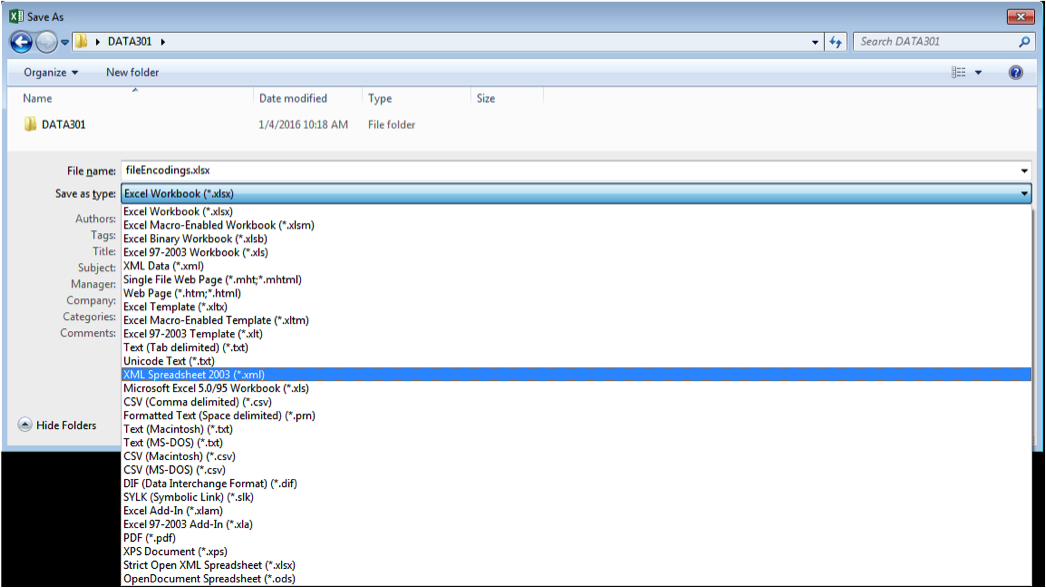
\includegraphics[width=.9\textwidth]{TryItFileEncoding.png}
\end{frame}


\begin{frame}{Opening xlsx in Excel}
\begin{exampleblock}
{Exercise:} Use the {\bf fileEncodings.xlsx} file and save the file as {\bf CSV}, {\bf tab-separated}, and {\bf XML}.  Look at each file in a text editor.
\end{exampleblock}
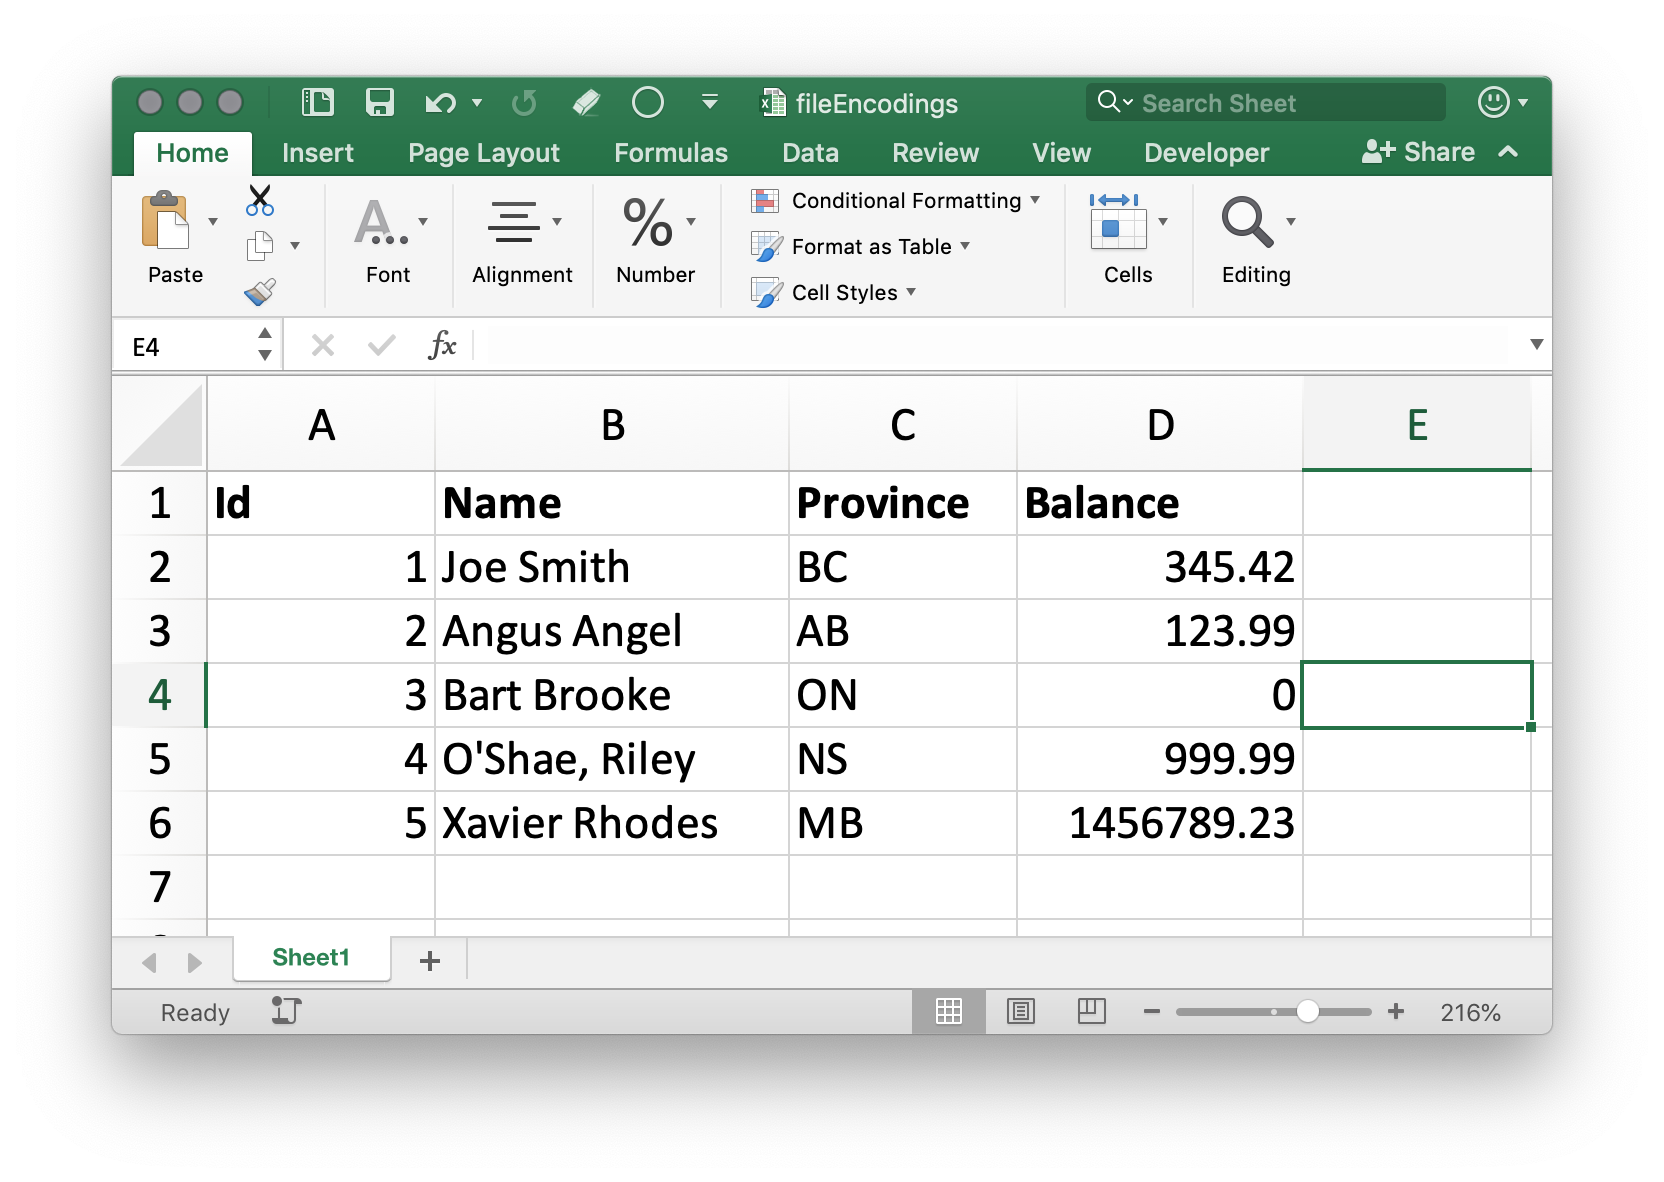
\includegraphics[width=.9\textwidth]{inExcel}
\end{frame}

\begin{frame}{Opening csv in text editor}
\begin{exampleblock}
{Exercise:} Use the {\bf fileEncodings.xlsx} file and save the file as {\bf CSV}, {\bf tab-separated}, and {\bf XML}.  Look at each file in a text editor.
\end{exampleblock}
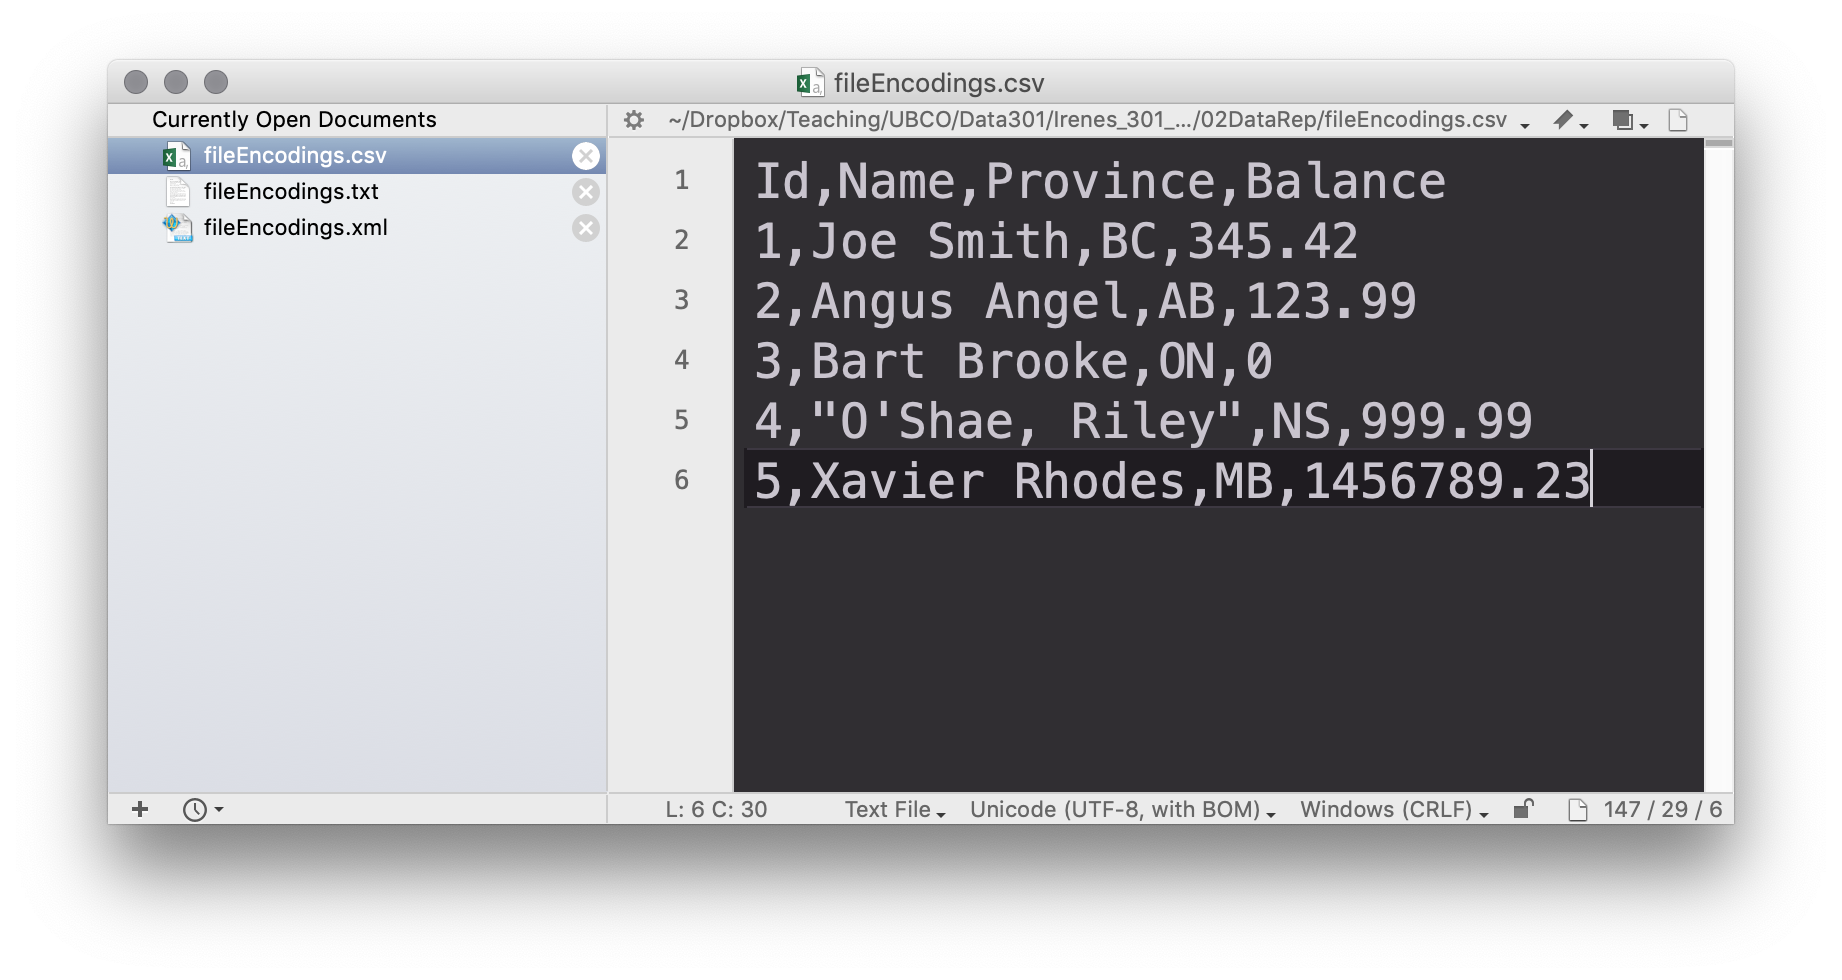
\includegraphics[width=.9\textwidth]{csv}
\end{frame}

\begin{frame}{Opening tab-separated in text editor}
\begin{exampleblock}
{Exercise:} Use the {\bf fileEncodings.xlsx} file and save the file as {\bf CSV}, {\bf tab-separated}, and {\bf XML}.  Look at each file in a text editor.
\end{exampleblock}
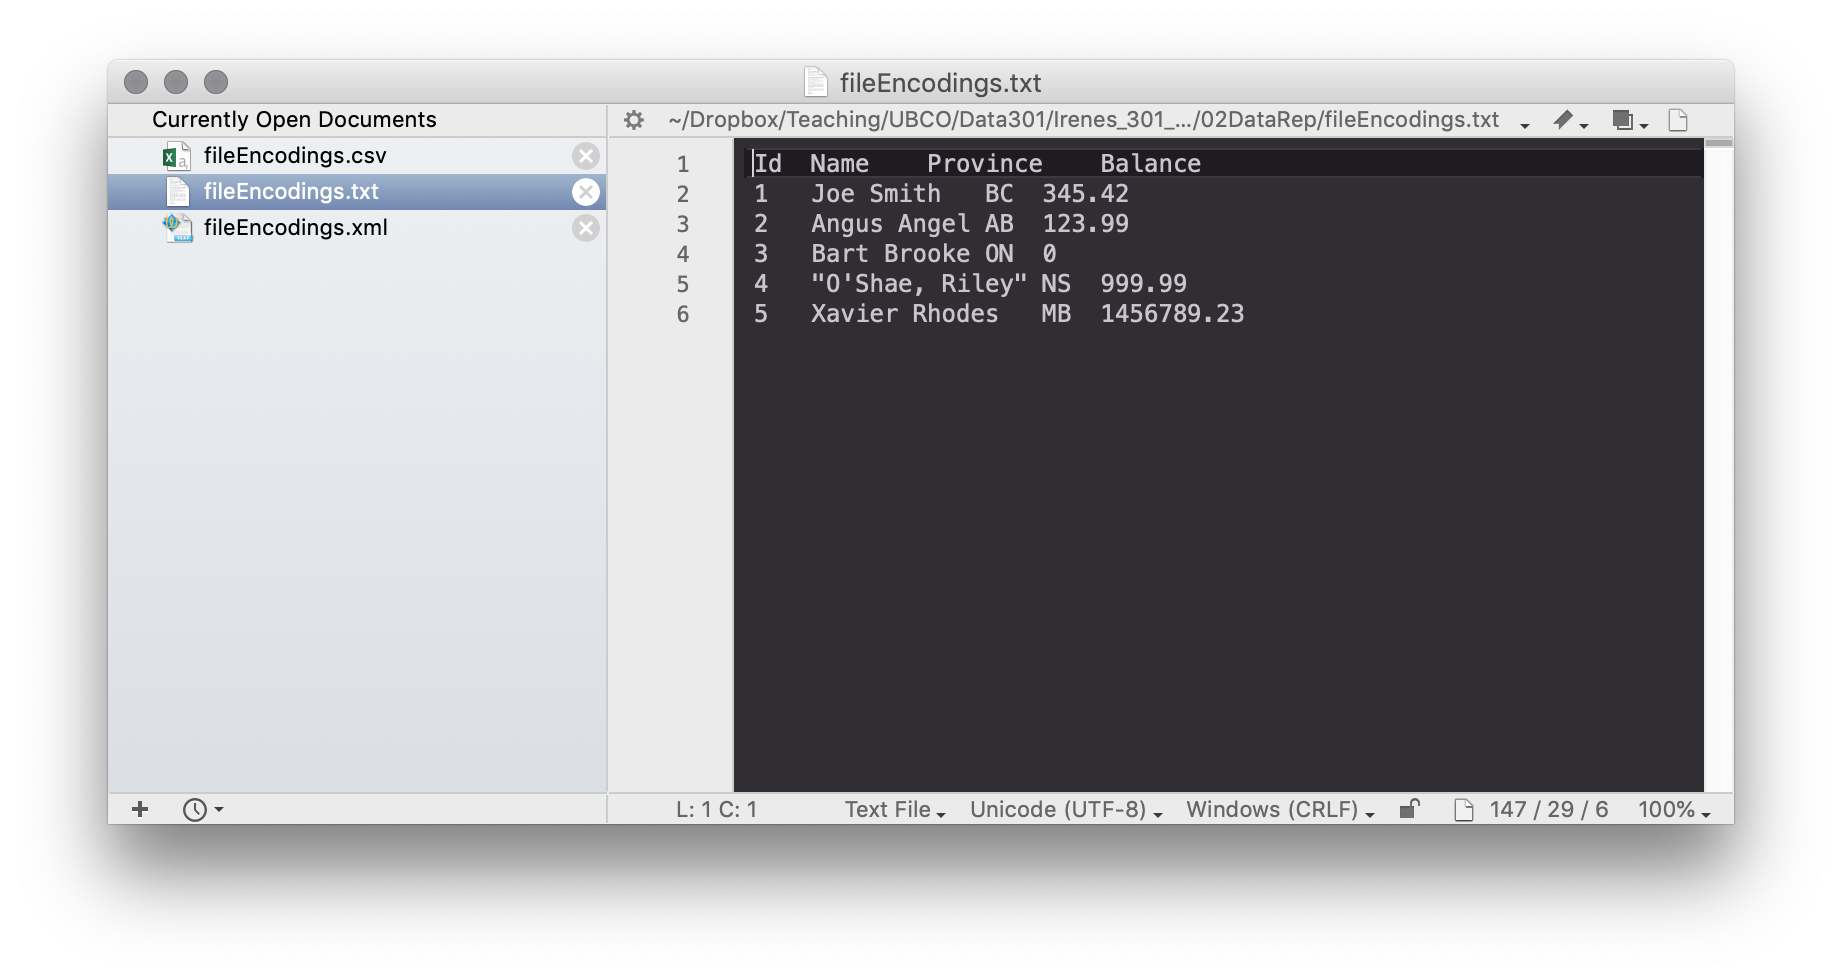
\includegraphics[width=.9\textwidth]{tabdelimit}
\end{frame}

\begin{frame}{Opening xml in text editor}
\begin{exampleblock}
{Exercise:} Use the {\bf fileEncodings.xlsx} file and save the file as {\bf CSV}, {\bf tab-separated}, and {\bf XML}.  Look at each file in a text editor.
\end{exampleblock}
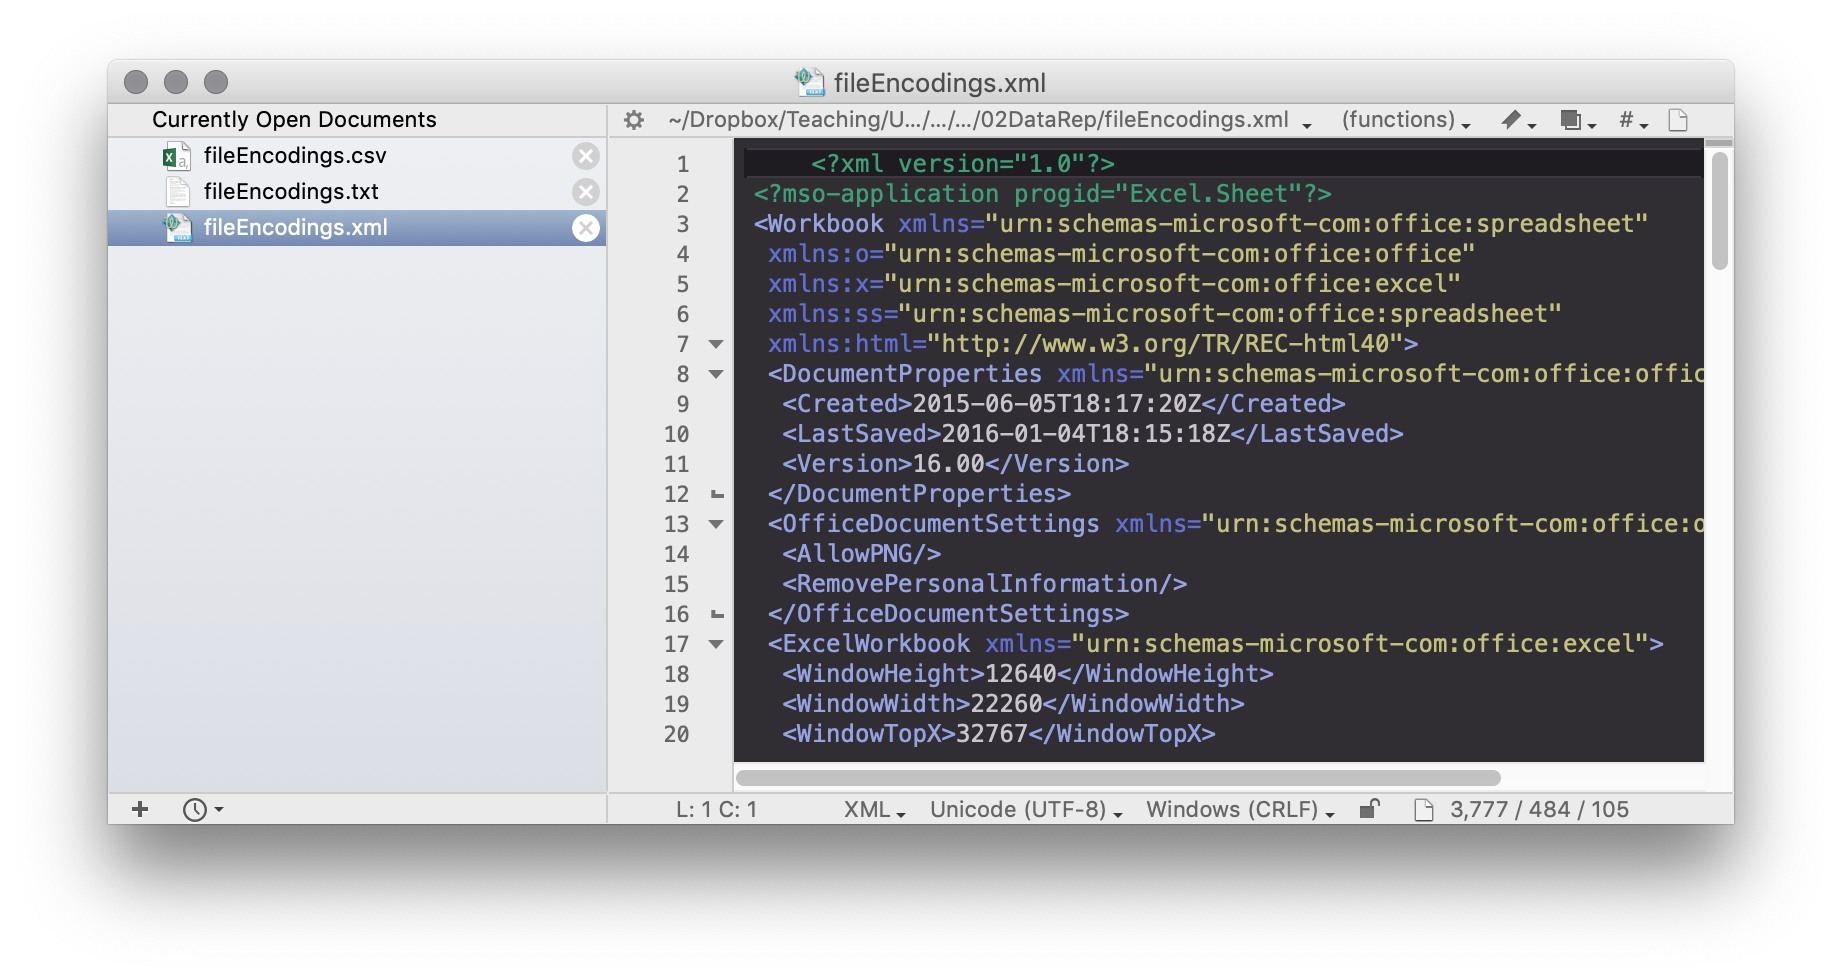
\includegraphics[width=.9\textwidth]{xml}
\end{frame}




\begin{frame}{UPC Barcodes}
\emph{Universal Product Codes (UPC)} encode manufacturer on left side and product on right side.  Each digit uses 7 bits with different bit combinations for each side (can tell if upside down).
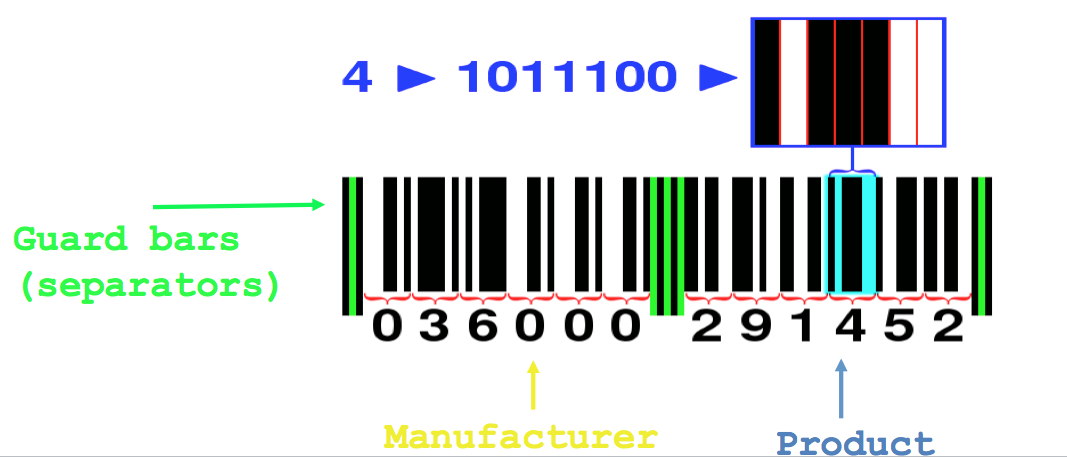
\includegraphics[width=.9\textwidth]{UPCbarcode.png}
\end{frame}

\begin{frame}{QR code}
A \emph{QR} (\emph Quick \emph Response) code is a 2D optical encoding developed in 1994 by Toyota with support for error correction.
\begin{center}
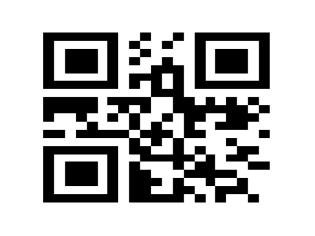
\includegraphics[width=0.3\textwidth]{QR1.png}\medskip
\end{center}
Make your own codes at: \url{www.qrstuff.com}.
\end{frame}


\begin{frame}{NATO Broadcast Alphabet}
The code for broadcast communication is purposefully inefficient, to be distinctive when spoken amid noise.\medskip
\begin{center}
\begin{tabular}{llllll}
A  & 	Alpha	  & 	J & 	Juliet		 & S 	 & Sierra	\\
B  &  	Bravo & 		K & 	Kilo	 & 	T & 	Tango\\
C  	 & Charlie	 & 	L & 	Lima		 & U & 	Uniform\\
D  & 	Delta	 & 	M & 	Mike		 & V & 	Victor\\
E   & 	Echo	 & 	N & 	November	 & W & 	Whiskey\\
F  & 	Foxtrot & 		O & 	Oscar 	 & 	X	 & X-ray\\
G    & 	Golf	 & 	P & 	Papa  & 		Y	 & Yankee\\
H & 	Hotel 	 & 	Q & 	Quebec	 & Z & 	Zulu\\
I & 	India		 & R	 & Romeo & 
\end{tabular}
\end{center}
\end{frame}

\begin{frame}{Advanced: The Time versus Space Tradeoff}
A fundamental challenge in computer science is encoding information efficiently both in terms of space and time.\\[1em]\medskip

At all granularities (sizes) of data representation, we want to use as little space (memory) as possible.  However, saving space often makes it harder to figure out what the data means (think of compression or abbreviations).  In computer terms, the data takes longer to process.\\[1em]\medskip

The \emph{time versus space tradeoff} implies that we can often get a faster execution time if we use more memory (space).  Thus, we often must strive for a balance between time and space.
\end{frame}

\begin{frame}{Review: Memory Size}
\begin{example}
 Which is bigger?
\begin{enumerate}[A)]
\item 10 TB
\item 100 GB
\item 1,000,000,000,000 bytes
\item 1 PB
\end{enumerate}
\end{example}
\end{frame}
%
\begin{frame}<handout:0>{Review: Memory Size}
\begin{block}{Answer:} Which is bigger?
\begin{enumerate}[A)]
\item 10 TB \emph{=10,000 GB}
\item 100 GB
\item 1,000,000,000,000 bytes \emph{= 1000 GB}
\item \yellow{\it 1 PB} \emph{= 1,000,000 GB}
\end{enumerate}
\end{block}
\end{frame}


\begin{frame}{Review: Metadata vs. Data}
\begin{example} How many of the following are TRUE?
\begin{itemize}
\item It is possible to have data without metadata.
\item Growth rates of data generation are decreasing.
\item It is possible to represent all decimal numbers precisely on a computer.
\item A character encoded in Unicode uses twice as much space as ASCII.
\end{itemize}
\begin{multicols}{5}
\begin{enumerate}[A)]
\item 0
\item 1
\item 2
\item 3
\item 4
\end{enumerate}
\end{multicols}
\end{example}
\end{frame}


\begin{frame}<handout:0>{Review: Metadata vs. Data}
\begin{block}{Answer:}How many of the following are TRUE?
\begin{itemize}
\item {\color<1->{Green}{It is possible to have data without metadata.}}
\item {\color<2->{red}{Growth rates of data generation are decreasing.}}
\item {\color<3->{red}{It is possible to represent all decimal numbers precisely on a computer.}}
\item {\color<4->{Green}{A character encoded in Unicode uses twice as much space as ASCII.}}
\end{itemize}
\begin{multicols}{5}
\begin{enumerate}[A)]
\item 0
\item 1
\item \yellow{\it 2}
\item 3
\item 4
\end{enumerate}
\end{multicols}
\end{block}
\end{frame}

\begin{frame}{Conclusion}
\begin{itemize}
\item All \emph{data} is encoded as bits on a computer. 
\item  \emph{Metadata} provides the context to understand how to interpret the data to make it useful.
\item Memory capacity and data sizes are measured in bytes.
\item \emph{Files} are sequences of bytes stored on a device.  A \emph{file encoding} is how the bytes are organized to represent data
\begin{itemize}
\item Text files (comma/tab separated, JSON, XML) are often processed during data analytics tasks. 
\item Binary files are usually only processed by the program that creates them.\medskip
\end{itemize}
\end{itemize}
As a data analyst, understanding the different ways of representing data is critical as it is often necessary to transform data from one format to another.
\end{frame}

\begin{frame}{Objectives}
\begin{itemize}
%\item Explain why it is important to understand and use correct terminology.
\item Define: computer, software, memory, data, memory size/data size, cloud
\item Explain "Big Data" and describe data growth in the coming years.
\item Compare and contrast: digital versus analog
\item Explain how integers, doubles, and strings are encoded.
\item Explain why ASCII table is required for character encoding.
\item Explain why Unicode is used in certain situations instead of ASCII.
\item Explain the role of metadata for interpreting data.
\item Define: file, file encoding, text file, binary file
\item Encode using the NATO broadcast alphabet.
\item Discuss the time-versus-space tradeoff.
\end{itemize}
\end{frame}

%\begin{frame}
%
%  \bibliographystyle{plain}
%\bibliography{../demo}
%
%\end{frame}

\end{document}

